\documentclass{UoYCSproject}
\usepackage{nameref}
\usepackage{longtable}
\usepackage{float}
\usepackage{graphics}
\usepackage{lscape}
\usepackage{enumitem}

\addbibresource{bibliography.bib}
\author{Robert Watts}
\title{Digital Charity Governance}
\date{Version 5, \today}
\supervisor{Simon Foster}
\BEng


\dedication{For Sue and Malcolm Watts}

\acknowledgements{
    Thank you to my supervisor Simon Foster for reading and providing feedback for my many drafts. Thank you to my family and housemates for keeping me sane (and for listening to me waffle about obscure nuggets of charity law).
}

\begin{document}
\pagenumbering{roman}
\maketitle
\listoffigures
\listoftables

% \renewcommand*{\lstlistlistingname}{List of Listings}
% \lstlistoflistings

\chapter*{Executive Summary}
\addcontentsline{toc}{chapter}{Executive Summary}  


There are over 168,033 charities in the UK, which are overseen by the Charity Commission \cite{commission_report_2022}. A charity is run by trustees who are responsible for ensuring that it follows governmental and regulatory compliance regulations. To aid the trustees in making good decisions, every charity must have a governing document describing how it should be run. In cases where the trustees fail to comply with regulations, the Charity Commission opens an investigation in which they inspect the minutes of trustee meetings to help them understand their decision making process. This shows that the minutes of any trustee meetings are paramount in proving a that a charity is compliant with the law. Therefore a tool that models a charity as a discrete system and allows trustees to minute meetings while checking they are following the rules of the charity could be created. 

A website makes the most sense for implementing this, because they can implement a Object Relational Map (ORM) model. A ORM model is a way of modeling real world entities, there is a series of database tables and logical classes that contain the functions (and validation rules) to manipulate the database. The website has two elements: a front end containing the user interface and a back end containing the model (in the ORM format) for the charity, along with the checks to ensure compliance. A series of existing web frameworks have been written to support website development and the best options for this project were Laravel (written in PHP) for the back end and React (written in Javascript) for the front end.

In implementing the website, it was necessary to select a specific governing document to analyse and tailor the tool, for an example governing document provided by the charity commission for a Charitable Incorporated Organisation \cite{charity_constitution_cio}. The first implementation step was to create the database structure. For this, Maria DB was used as it provided the best performance. After this the charity model was created within Laravel, after which the API routes were designed and a way of storing meeting attendance implemented. Within the API routes is also where the compliance checking takes place. Finally a front end user interface was created that consumed the API. This used various other modules to support the React framework in creating pages and data handling. 

To validate that the model was created correctly and that the front end behaves as expected a series of both unit tests and manual tests were created. These were primarily based around a series of requirements that had been written before the website had been implemented. In total 20 unit tests were written (achieving a code coverage of 81.82\%) and 16 manual tests were written and run. Due to time constraints it was not possible to complete all of the requirements that were created, however the vast majority were implemented to some degree. This all showed that it was indeed possible to model a charity successfully and create an interface that allows the model to be manipulated. 

For the most part the project went smoothly however there are some bits that require further work and investigation. The biggest of these was that throughout this project no questionnaires or usability studies were conducted with charity trustees and members. For this reason the project cannot categorically conclude that the tool that was created supports charities in the best possible way, however it has instead showed that a charity model could be created.

None the less, the project was successful in achieving the aims it set out to.


\chapter{Introduction}
\label{cha:introduction}
\pagenumbering{arabic}


The charity sector in the UK has grown substantially in the last decade, now being worth over £83.8 billion \cite{commission_report_2022}. Which such inordinate amounts of money flying around it is only right that the public demand a certain level of public scrutiny of the charity sector. Despite this however, charities are finding themselves under ever increasing demand for their services (especially as the cost of living crisis in the UK gets worse \cite{butler_2023}), further putting strain on the selfless and dedicated trustees that run the charities. None the less, running a charity is not always easy, governmental and regulatory compliance are a minefield to navigate for both new and experienced trustees alike.

The aim of the project is to explore how charities can benefit from software that provides compliance checks by creating a proof of concept to software system to prove that a digital model of a charity can be formed.

The projects main objectives are as followed:
\begin{itemize}[noitemsep]
    \item Establish what the issues charities (and their trustees) currently face and how technology can be used to support them
    \item Formulate a comprehensive list of requirements
    \item Define a model of a charity that can be used within a computer system
    \item Apply that model to create a software tool that can support trustees
    \item Evaluate the effectiveness of the implemented software 
\end{itemize}

If all these objectives are met then it shows that a suitable charity model can be formulated and as a consequence, computerised systems can be used to support charities.


\chapter{Literature Review}
\label{cha:litreview}

This chapter reviews existing literature, laws, and methodologies that currently exist in the charity and application development spaces. It has been split in too three phases; The first phase will look at the charity sector in the UK, including the laws and other regulations that govern how charities should run. This section should give a good grounding for what compliance checks the tool will need to complete. The second phase will look at cases where charities have failed previously and will try to see what lessons can be learnt from them. This should hopefully give an idea as to how a digital charity model can be used to support charity governance. The final phase will look at application development, and what tools exist to create the model of a charity. If done successfully this phase should find tools and methodologies that are currently used to model real world entities, and are also applicable to this project.

\section{The Charity Sector in the UK}
In 2017 the charity sector in the United Kingdom had an income £76 billion \cite{commission_report_2017} and by 2022 that had risen to £83.8 billion \cite{commission_report_2022}. The majority of charities are small, 75\% have income less than £100,000 per year \cite{value_of_charity_sector_2017}. With such inordinate amounts of money being raised by charities via fundraising, donations, investments and trading (sales) income, the sector has to be closely monitored. With over 168,033 charities in England and Wales (in 2022), being run by 700,000 individual trustees \cite{commission_report_2022} His Majesty's Government (HMG) has delegated this responsibility to the Charity Commission, a non-ministerial government department. Although the United Kingdom has had a permanent body governing the rules surrounding the registration and regulation of charities since the Charitable Trusts Act of 1853 \cite{national_archives_1853_1960}, it was not until the Charities Act of 2006  \cite{charities_act_2006_introduction} (and later extended in the Charities Act of 2011) when the Charity Commission, as we know it today was formed. 

As well as forming the Charity Commission (and providing them with regulatory powers) the Charities Acts of 2006 and 2011 also brought in new requirements that charities must meet before they are able to become a charity. The first of these surround the charity itself: the charity must be for the public benefit \cite{charities_act_2011_section_4_public_benefit}. This means that the charity must fit into one of the following categories \cite{charities_act_2011_section_3_purpose}:
\begin{itemize}[noitemsep]
    \item The prevention or relief of poverty
    \item The advancement of education
    \item The advancement of religion
    \item The advancement of health or the saving of lives
    \item The advancement of citizenship or community development
    \item The advancement of the arts, culture, heritage or science
    \item The advancement of amateur sport
    \item The advancement of human rights, conflict resolution or reconciliation or the promotion of religious or racial harmony or equality and diversity
    \item The advancement of environmental protection or improvement
    \item The relief of those in need, by reason of youth, age, ill-health, disability, financial hardship or other disadvantage
    \item The advancement of animal welfare
    \item The promotion of the efficiency of the armed forces of the Crown, or of the efficiency of the police, fire and rescue services or ambulance services
    \item Any other charitable purposes
\end{itemize}

Once the charity has been deemed to be of public benefit, the next requirements surround the governing document (or constitution) - namely that there must be one. The Charities Act of 2011 states that the governing document should include the charities name, purpose, who is eligible for membership, how a person becomes a member, how trustees are appointed and any conditions of eligibility for their appointment, and finally what should happen to the property and assets of the charity in the event that it is dissolved \cite{charities_act_2011_section_206_governing_doc}. The document should also include how trustee meetings should be conducted, and what quorums (if any) are required \cite{charities_act_2011_section_223_trustee_responsibilities}.As the vast majority of charities have similar requirements the charity commission provides 7 different types of example documents for charities of different sizes and legal structures \cite{gov_uk_example_trustee_docs}. The charities act states that trustees must follow their charities governing document \cite{charities_act_2011_section_223_trustee_responsibilities}. 

The next set of requirements relate to the trustees that are defined in the governing document. A trustee must be 16 years old for a charity company or charity incorporated organisation, or 18 for all other types of charity \cite{essential_trustees_guide}. They also cannot have been disqualified. Sections 178 through 184 of the 2011 Charities act defines the full reasons why someone may not be a trustee, some examples of these are a trustee can not have ever declared bankruptcy, they must not have any unspent convictions and they must not be on the sex offender register \cite{gov_uk_disqualifying_reasons}. The latter two of these are particularly important, because for any charity that works with children or vulnerable adults, the trustees must also pass a Disclosure and Barring Service (DBS) check to look at their criminal record \cite{essential_trustees_guide}.  The final requirement, should the charity want to claim gift aid (an extra 25\% on any donation to the charity), then the trustees must also pass His Majesty's Revenue and Customs (HMRC) Fit and Proper Test, to ensure that the gift aid funds will not be subject to tax fraud \cite{hmrc_fit_and_proper_test}. 

Charities must also keep strong financial records. The rules for a charity vary depending on how much income the charity generates each year. A charity whose yearly income is less than £10,000 only needs to provide the charity commission with very basic accounting information while a charity whose yearly income is over £10,000 needs to provide a full set of accounts \cite{essential_trustees_guide}. On top of this requirement any charity whose income is over £25,000 needs to provide a trustees annual report detailing the charity's work (its aims and objectives throughout the year), where the charity's income has come from and how the money has been spent \cite{gov_uk_annual_report_doc}. While the trustees can delegate responsibility to employees or other volunteers within a charity to produce all these documents, if the charity fails to provide them it is a criminal offence for which the trustees can be held liable \cite{essential_trustees_guide}.

One key thing that the Charity Act brought in was the liability that trustees have for the charities they run \cite{charities_act_2011_section_191_liabilities}. The guidance provided by the Charity Commission is that if a charity has been formed by an unincorporated legal structure, (which most small charities are) such as a Trust or Association, then the trustees of the charity are not indemnified from any mistakes that they make \cite{essential_trustees_guide}. In practice this means that any legal issues or lawsuits that arise during the running of the charity, are personally liable to the trustees and not the charity. For this reason, it is very much in the interest of the trustees to ensure that their charity is run in a manner that is compliant with the Charity Commission's rules, but it is also important that they ensure that their charity is being run with good governance practices.

Jones and Hyndman argue that defining governance for charities is harder than the business sector. However, one of the central things that they point out (among other things) is that whatever governance practices trustees choose to follow, they should be accountable to both donors (as without their support the charity does not exist), volunteers, and beneficiaries \cite{hyndman_jones_2011}. In all three of these cases both Jones and Hyndman and the Charity Commission say that charities should live within their means; that is they shouldn't over-commit resources \cite{essential_trustees_guide}\cite{hyndman_jones_2011}. For this reason, the Charity Commission recommends that charities follow the Charity Governance Code to ensure that good governance practices are followed \cite{essential_trustees_guide}. Indeed, this code concurs with Jones and Hyndmans stating in section 7.1 of the code that “The organisation’s work and impact [should be] appreciated by all its stakeholders” \cite{charity_governance_code_2020_section_7}. 

If good governance practices are not followed, the Charity Commission are within their rights to open an investigation. In 2018-2019, 2269 \cite{commission_report_2019} of these investigations were started by the charity commission. In extreme cases where there has been a governance failure (or criminal activity such as fraud) the Charity Commission will start a statutory enquiry which allows it to obtain evidence and use enforcement powers to protect assets \cite{essential_trustees_guide}.

From understanding the structure of charities and the definition of good governance it should be possible to formulate a model of a charity. It is clear that charities may exist within a discrete system of states and that as the trustees make decisions, they move between these states. From this section a determination can be made as to which states are compliant with the law and which ones are are not. When charities are not compliant however, charities are investigated, so it will be useful to see which of these states are important when it comes to non-compliance.

\section{Cases of Governance Failures} \label{chap:charity_governance_failures}
The charity commission publishes most completed charity commission investigations on their website, which makes for a fairly large dataset of serious breaches of the Charities Act of 2011 \cite{gov_uk_commission_alerts}. This project has looked into two of these in more detail.

\subsection{The Retreat Animal Rescue}
The Retreat Animal Rescue was registered in April 2004 and they aim ‘to relieve the suffering of unwanted, abandoned and neglected animals that are in need of care and treatment, by the provision of a rescue and re-homing service and the accommodation of such animals, and to advance public education in matters concerning animal welfare’ \cite{animal_rescue_report}. In the 2020-2021 financial year they had an income of £298,890 meaning they are a medium sized charity \cite{animal_rescue_finance}. In 2018 the charity commission started an investigation into the charity as they had not complied with their obligations under the charities act 2011, by failing to submit their annual accounts and returns in the financial years ending in 2016, 2017 and 2018. Not only was this a breach of the law, but broke a clause in their governing document that stated that the charity must file its financial information \cite{animal_rescue_report}. 

While the charity commission were investigating, they found that the charity was in breach of their governing document, between September 2015 and April 2020, by only having four trustees and not the 5 required by the document \cite{animal_rescue_report}. 

The final governance issue that the Charity Commission found was that the charity received a £200,000 donation and entered into a 25 year lease for property (using the donation for the prepayment). The charity could not enter into this lease under their own governing document as it did not have enough trustees. On top of this, one of the trustees was the one leasing out the land, and as the charity was unincorporated, signed both sides of the lease. The commission stated in their report that “It is not legally possible to enter into a contract with yourself, consequently, the inquiry found that there are significant doubts about whether the lease is legally valid.”\cite{animal_rescue_report}

This was a conflict of interest that was not declared by the trustee involved, which was against the law and governing document of the charity. This trustee therefore resigned and the charity was given an action plan to sort out the other issues. Official warnings were also given to other trustees within the charity\cite{animal_rescue_report}.


\subsection{The Ashley Foundation}
The Ashley Foundation was registered in May 1997 to provide hostels and flats for homeless people. Its stated aim was to support “the relief of poverty by the provision of accommodation to persons in need and in such other ways as the trustees think fit.” \cite{ashley_foundation_report}. They are a large charity and in the 2021-2022 financial year (after the investigation) had an income of £3.66 million \cite{ashley_foundation_finance}. 

Issues were raised to the charity commission by trustees in 2019 regarding the sale of property owned by the charity, as well as the amount of money reimbursed to the CEO of the charity over the preceding few years. In the winter of 2017 the charity sold three properties to a company for £4 million, and that company then sold them later that same day for £6.4 million. 

The charity commission used minutes from October and November of 2017 to determine if this sale was legal, as the property was undervalued. They were not able to find "any minutes that recorded the terms of the Agreements being discussed by the trustees or that the risks, obligations, and liabilities of entering into them had been considered in advance of the Agreements being signed” \cite{ashley_foundation_report}. During the investigation the charity commission found that the CEO had received a payment of £40,000 for his role in the sale of the properties \cite{ashley_foundation_butler_2023}. 

While this was under investigation it then subsequently came to light that the CEO had also been reimbursed for over £840,000 including the purchase of Apple IPhone's, Apple Watches, Dyson Supersonic Hairdryer, first class travel (inc hotels, food and accommodation) and tracking software \cite{ashley_foundation_bbc}\cite{ashley_foundation_report}. 

The charity commission found that there were serious breaches of mismanagement in the governance of the charity. Three of the trustees were removed from the charity and the CEO was later jailed after the investigation was referred to Lancashire police for fraud\cite{ashley_foundation_report}.

\subsection{Lessons to be Learnt}
From both the Ashley Foundation and the Retreat Animal Rescue it is clear that the trustees had not complied with either the law or the charities own governing documents. What is important to note in both of these cases however, is that throughout the investigations the charity commission undertook, the minutes of the trustees meetings were of immense importance in determining the decision making process of the trustees. Ensuring an accurate record of meetings is essential for ensuring good and transparent governance and so it is clear that a tool that supports the governance of meetings would be the best use of this project.
https://www.overleaf.com/project/63dfe9c9c80dad22d4a8eada
\section{Web Application Development}
\label{sec:web_app_dev}
The user will need some way to interface with the tool. This could be done via a Desktop app, Mobile App or a website. There are pros and cons to each, however this project will focus around web app because they can be accessed via any browser on mobile and desktop \cite{tuama_2022}, meaning it suits the requirements of both.

There are two parts to a web application, server side and client side. The American cyber security company Cloudflare Inc defines client side as “everything in a web application that is displayed or takes place on the client using Markup languages like HTML and Cascading Style Sheets (CSS)" and they define server side as everything that happens on the server which can include “nearly all business logic [running] on the server side, and this [includes] rendering dynamic web pages, interacting with databases, identity authentication, and push notifications” \cite{cloudflare_client_vs_server_side}. Having logic run on the back end of the website (as opposed to a static website) allows the content of the pages to be changed for every user based on their stored preferences in the database \cite{muittari_2020}.

More modern websites however change this model slightly by using Javascript to render information pulled from an application programming interface (API) on the client side. An API allows developers to access data and services to help rapidly build websites and applications. This updated model allows for content on the website to be more flexible and allows for a better technical architecture, as it allows for only the information required to be gathered from the database, reducing the overheads. This model is used extensively by many companies but Facebook and Twitter are good examples \cite{jacobson_brail_woods_2012}. Facebook traffic accounts for 25 percent of all page views on the internet and API’s are extensively used within their ecosystem; indeed Facebook has over 5 billion calls per day \cite{jacobson_brail_woods_2012}.

Regardless of which back end architecture some form of server side programming is required. In broad terms, these scripts need to take in a HTTP request, then access the database and return some output (either HTML or an API response) \cite{muittari_2020}. To make this process easier developers can use web frameworks. These provide URL’s that call handler functions to manipulate the data in some way. They also provide tools for common tasks such as “session handling, user authorization, security against malicious attacks and output formatting”\cite{muittari_2020}. A particularly key function of frameworks is that they need to provide a way for web applications to store data within a database. 

Most frameworks use an abstraction layer called Object-Relational Mapper (ORM) to do this. A ORM model is a way of modeling real world entities, there is a series of database tables and object oriented classes that contain the functions to read, write, query, and delete data. This has two advantages, it means the developer has to write less SQL code and it makes applications development faster \cite{techopedia_orm_definition}.

There are many back end frameworks that provide these functionalities in a variety of languages. They all have different pros and cons; indeed a quick google will find a variety of opinion pieces arguing which one is “best”. Rather than trying to find the “perfect” framework a better method was to look for the most popular, the assumption being that this would provide the best resources for me later in the project. Every year the programming question and answer website Stack Overflow does a survey of all its members and found that the top back end web framework among professional developers was ExpressJS \cite{stackoverflow_dev_survey_2021}. This is an imperfect metric as it requires people to have responded to their survey, so the website statisticsanddata.org ranked them by the number of stars (“likes”) that each framework has on the social code platform Github \cite{statisticsanddata_backend_frameworks_2021} in the month January 2022. The graph produced by them is shown in figure \ref{fig:statisticsanddata}

\begin{figure}[htb]
\begin{center}
\includegraphics[height=6cm]{"./assets/lit-review-assets/statisticsanddata_backend_frameworks_2021_2022"}
\label{fig:statisticsanddata}
\end{center}
\caption{The most popular back end frameworks in January 2022 ranked by Github Stars \protect\cite{statisticsanddata_backend_frameworks_2021}.}
\end{figure}

Looking at the top 4, Laravel uses PHP and follows the ORM model discussed above \cite{otwell_2015}. Django and Flask are both written in python, however while Django includes the ORM model for database access within the module \cite{django_docs}, Flask does not and extra plugins are required \cite{flask_docs}. The final one, ExpressJS (which was also mentioned in the Stack Overflow developer survey), is just a web server that helps structure and route the application. To do much more you need to install plugins for everything via NPM (a Node package manager), so it makes it flexible enough to follow the ORM model \cite{vivah_2019}. 

While the back end framework can provide the data to an application via an API the data still needs to be displayed on the client's device (on the front end). To do this a front end framework can be used. These provide tools for rapid development, as well as aim to achieve features and applications that are more responsive than more traditional applications \cite{monocubed_2021_best_frontend_frameworks}. There are a lot of these and to determine the most used ones by developers, the web development agency Monocubed ranked them by the number of stars (“likes”) that each framework has on the social code platform Github \cite{monocubed_2021_best_frontend_frameworks}. This data can be seen in table \ref{table:monocubed_2021_best_frontend_frameworks}.


\begin{table}[H]
\begin{center}
\label{table:monocubed_2021_best_frontend_frameworks}
\resizebox{7.175cm}{!}{%
\begin{tabular}{ll}
\hline
\textbf{Framework}    & \textbf{Github Stars} \\ \hline
React Framework       & 192K                  \\ \hline
Angular Framework     & 83k                   \\ \hline
Vue.js Framework      & 198k                  \\ \hline
Ember.js              & 22.2k                 \\ \hline
jQuery                & 56.5k                 \\ \hline
Semantic-UI Framework & 50.1k                 \\ \hline
Backbone.js           & 27.9k                 \\ \hline
Preact Framework      & 32.5k                 \\ \hline
Svelte Framework      & 61.1k                 \\ \hline
Foundation            & 29.3k                 \\ \hline
\end{tabular}
}
\caption{ The number of Github stars of popular front end frameworks front end frameworks 
\protect\cite{monocubed_2021_best_frontend_frameworks} }

\end{center}
\end{table}

From this we can see that React Framework and Vue.js Framework are the two most popular. React allows you to build encapsulated components, each of which has their own state. These components can then be combined to build bigger and bigger components until you end up with very high level ones \cite{react_docs}.  In contrast Vue.js uses a template model in which data is input into templates. Vue.js however has not been around as long as other frameworks and therefore lacks experienced developers \cite{goncharenko_2022}. 

For both the front end and back end maintainability is important, meaning that the number of developers that can use particular languages is key. In the Developer Nations “State of the Developer Nation” report they attempted to assess which were the most widely used programming languages \cite{korakitis_muir_jones_condon}. This can be seen in figure \ref{fig:developer_nation} and from this I can see that Javascript, Python, and Java are the most commonly used languages. This means that when selecting a framework it will be important to choose one that uses one of these languages. 

\begin{figure}[htb]
\begin{center}
\includegraphics[height=7cm]{"./assets/lit-review-assets/developer_nation_programming_languages"}
\label{fig:developer_nation}
\end{center}
\caption{The number of active software developers back end programming languages in Quarter 1 of 2022. \protect\cite{korakitis_muir_jones_condon}.}
\end{figure}

From this research it is clear that there are a verity of options for the development of both the front end and the back end website. The ORM model of development should support developing a charity model well, and as well as being quick for rapid prototyping. 

\chapter{Methodology}
\label{cha:methodology}
This chapter covers the methodology that the project used. It looks in depth at the requirements gathering, consideration of different design options and analysis of available languages and tools. From the research that has been gathered into the charity sector and web applications, it is clear that to ensure good governance that an accurate record of meetings are essential. Therefore once this project has created a model for a charity, it will use that model to implement a minute taking system that ensures compliance of charity votes.

This project is going to follow the Waterfall Method of development \cite{waterfall_method}. The Waterfall methodology is a sequential development process, where each phase of development takes you through the project. Much like a Waterfall, each phase must be fully complete before the next phase can start. Different projects have different exact stages, however the five most common ones are: 
Requirements, Design, Implementation, Verification or Testing, and Deployment and Maintenance. This state based methodology suits the project because each step is clearly defined and has clear goals before moving on to the next stage. This provides an straight forward order of operations to follow throughout the project.

This project does not explicitly look at the deployment of the system, therefore it will not be included in this diagram. This means that the Waterfall will look like figure \ref{fig:waterfall}. 

\begin{figure}[htb]
\begin{center}
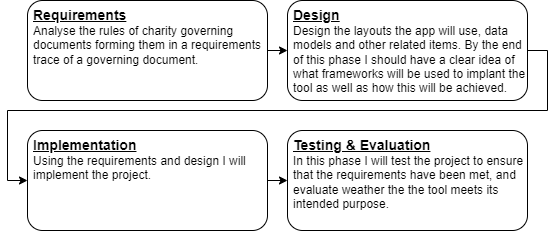
\includegraphics[height=5cm]{"./assets/methodology-assets/Waterfall v2.png"}
\label{fig:waterfall}
\end{center}
\caption{Proposed Waterfall method.}
\end{figure}




\section{Design Options}
To determine the requirements of the project, the scope needs to be defined. There are 3 options when it comes to the scope:

\textbf{Option 1} - The first option is to create a tool that aims to support the meetings of specific charity sectors (i.e. Student Unions, NGO's, Food Banks, etc). For example the meetings held by the trustees of a Scout Group would look substantially different to the meetings held by a Food Bank. The sector would have to be chosen quite carefully to provide a set of features that actually support the governance of the charities rather than hinder them. There are already a series of tools that look at this, so while this type of tool could be useful to charities and support their governance and work, this is not the best use of this tool. 

\textbf{Option 2} - The second option is to create a tool that will support the implementation and governance of a specific charities governing document. This would provide the most scope for this investigation to see how charities could benefit from a technological solution, however this advantage is also a limitation - because it would be limited to this one charity document the investigation would not be representative of all charities in the UK.

\textbf{Option 3} - The third option is to create a tool that will support the governance of any charity regardless of the governing document. Users would have to input information about their charity, governing document and membership, and then the tool could support their governance based off these inputs. This would be the most generic tool of all the options. The ability of a tool to do everything often means that it does everything poorly, and I believe that this would be no different; that is to say it would be complex to create a tool that suits all governing documents well.

\textbf{Conclusion} - All three of these options have their pros and cons, however option 2 has been chosen for this project. This is because it provides the best opportunity to show that a charity can benefit from digital governance. A single governing document provides a limited scope to analyse and work off. If this tool is successful future research could the build off this research to look into Option 3. So that the governing document chosen has the best chance of being applicable to the most charities possible, an example governing document provided by the Charity Commission has been selected \cite{gov_uk_example_trustee_docs}, the decision for which is shown in the next section.

\section{Analysis Of A Governing Document}
\label{sec:analyisis_governing_doc}
A governing document should contain the process for how the charity should be run; it should contain everything from the charities name, membership processes, trustees and how meetings should be run. As we have seen in both of the governance failure case studies in chapter \ref{chap:charity_governance_failures}, the minutes of the meetings was used extensively to determine the thinking of the trustees at any given moment. For this reason, in the analysis of a governing document the focus will be on how technology can be used to support these meetings and therefore look more in-depth at how a trustee meeting should be run. 

So that the tool is applicable to as many charities as possible, the analysis is going to look at a model governing document produced by the Charity Commission, more specifically the model entitled: "Constitution of a Charitable Incorporated Organisation whose only voting members are trustees"\cite{charity_constitution_cio}. This Governing Document is for a Charitable Incorporated Organisation (CIO) which was a new legal structure for charities provided under the 2011 Charities Act \cite{charities_act_2011_section_204_cio}. A CIO is an incorporated structure that allows members to have limited liability for issues within the charity \cite{vistra_2019}. The constitution of these charities is prescribed by the Charity Commission and is therefore not as flexible as other charities \cite{vistra_2019}. This has advantages for the proof of concept tool this project is creating, as it means that it will apply to a large number of charities. The charity commission provides two model constitutions for CIO's for Foundations (where the only voting members are the trustees) and one for Associations (where members can vote). There are no clear statistics on how many there are of each type on the Charity Register, however this paper will look at the foundation model, as anecdotally while finding case studies for this paper, there have been more foundations. 

The document is quite long and to aid in understanding it, it was necessary to go through and summarise each clause in the document. There is more detail below regarding information about the document, however the full summarised version can be found in "\nameref{sec:apendix_1_gov_doc_sumary}". It is worth noting that in certain places the model governing document allows the reader to choose different processes for running the charity and as the project develops, a selection of these options will need to take place.

According to the governing document the charity is made up of trustees (clause 16). These trustees must be at least 16 years old, must not be disqualified under charities act and must accept the post willingly (clause 9). The number of trustees is variable however this simplest way of defining it is that there must be a minimum of 3 (clause 9). The election of new trustees must take place at a general meeting and the simplest way of selecting new trustees is for the existing trustees to elect them (clause 10). There are two main types of meetings: general meetings and trustee meetings. At general meetings (one of which must happen every year) amendments to the constitution, amalgamation with another charity and dissolution of the charity can be voted on, although these need at least 75\% of the electorate to pass (clause 18). In trustee meetings one person should be the chair, and resolutions should be voted on (clause 15). Clause 15 Sub section 3 says that decisions must have a quorum which is two charity trustees, or the number nearest to one third of the total number of charity trustees. Trustees should declare if they have a conflict of interest and should not vote in matters that conflict. In either type of meeting there must be minutes kept that contain a record of appointments of trustees, proceedings of general meetings, proceedings of charity trustee meetings (including who was present, any decisions made and the rationale behind those decisions). 

From this analysis of the rules around charity meetings, the requirements for the tool can be formed. This analysis has helped in creating requirements that ensure compliance is maintained. This analysis can also form the basis of testing that the tool is working correctly, as tests can be written for different parts of the governing document to ensure they are followed.

\section{Existing charity solutions}
From both the extent to which the minutes are talked about in the governing document and their use within investigations of charity misconduct, it is clear that the minutes of charity meetings are important. In theory the minutes should provide an accurate record of why any decisions were made. Consider the following examples: \textit{Student Union Management System (SUMS)} \cite{sums_website}, \textit{Online Scout Manager (OSM)} \cite{OSM_website}, and \textit{Magic Minutes} \cite{magic_minutes_website}. Each of these provides tools that empower charities to follow their governing documents.  As you can see in table \ref{table:existing_solutions} they all have different feature sets.

\begin{table}[]
\begin{center}
\caption{ Features of existing charity applications.}
\label{table:existing_solutions}
\begin{tabular}{llll}
\textbf{Feature}            & \textbf{SUMS} & \textbf{OSM} & \textbf{Magic Minutes} \\ \hline
Track charity membership    & Yes           & Yes          & No                     \\
Track charity finances      & Yes           & Yes          & No                     \\
Minute Meetings             & Yes           & No           & Yes                    \\
Membership Voting           & Yes           & No           & No                     \\
Trustee Elections           & Yes           & No           & No                     \\
Action Points from Meetings & No            & No           & Yes                    \\
Create Agendas              & Yes           & No           & Yes                   
\end{tabular}
\end{center}
\end{table}

As SUMS is aimed heavily at Student Unions, it has a lot of features around the democratic elections of trustees. With OSM the opposite is somewhat true because its main features relate to member management, and as a trustee in Scouting you are responsible for a large number of children. Because SUMS and OSM are aimed very much at their respective sectors (Student Unions and Scouting) they are not really useful to the wider charity sector, although individual features within them would be. Magic Minutes on the other hand is usable by a wide range organisations, almost to the point where it does not have enough features for charities. However, it is incredibly good at its single focus, minute taking, which is a feature that the charity sector could benefit from.

From this we can see that there is a lack of good tools that are designed for charities to take minutes. 


\section{Requirements For The Application}

The requirements for the product are shown in table \ref{table:requirements} on page \pageref{table:requirements}. To help  prioritise the requirements I will implement first, this project is going to use the MoSCoW method. This is a prioritization technique for prioritising requirements in which product objectives are put into 4 categories: \textit{Must Have}, \textit{Should have}, \textit{Could Have} and \textit{Will Not Have} \cite{MoSCoW_productplan_2018}. While developing this project lots of ideas have been considered but for brevity the \textit{Will Not Have} section has not been included in this document. 


\begin{table}[htb]
\label{table:requirements}
\begin{center}
\resizebox{\textwidth}{!}{%
\begin{tabular}{|p{0.07\textwidth}|p{0.2\textwidth}|p{0.66\textwidth}|}
  \hline
  \textbf{ID} & \textbf{Type} & \textbf{Requirement} \\\hline
  \multicolumn{3}{|c|}{\textit{\textbf{Must have}}} \\\hline

  1.1   &   Functional   & 
             The application must have a database containing charity meetings, the minutes, votes, and trustees   \\\hline
1.2   &   Functional   & 
             The application must take in the minutes of a meeting and return confirm that they are valid   \\\hline
1.3   &   Functional   & 
             A data structure should be created for a meeting that can be easily validated   \\\hline
1.4   &   Functional   & 
             A valid meeting should ensure that quorum is met for all votes   \\\hline
1.4.1   &   Functional   & 
             If it is a constitutional amendment then at least 75\% of members should vote for it to pass   \\\hline
1.4.2   &   Functional   & 
             If it is a resolution is up for vote the for it to pass it must have at least two charity trustees,
or the number nearest to one third of the total number of charity trustees, whichever is higher vote for it to pass   \\\hline
1.5   &   Functional   & 
             A user should be able to input markdown as plain text input for the minutes of a meeting   \\\hline
1.6   &   Functional   & 
             A user should be able to view meetings afterwards   \\\hline
1.7   &   Non-Functional   & 
             Code should be commented for future maintainability   \\\hline
1.8   &   Non-Functional   & 
             The application should be easy to use   \\\hline
1.9   &   Non-Functional   & 
             The application should display minutes and votes in an easy to understand format   \\\hline
 \multicolumn{3}{|c|}{\textit{\textbf{Should have}}} \\\hline
2.1   &   Functional   & 
             The application should allow for the election of new trustees to be included in the minutes of a meeting   \\\hline
2.2   &   Functional   & 
             The application should allow trustee resignations to be included in the minutes of a meeting   \\\hline
2.3   &   Functional   & 
             Each trustee has their own user account and can log in to view minutes of the meetings   \\\hline
2.4   &   Functional   & 
             The application should have separate rules for general meetings and trustee meetings   \\\hline
2.5   &   Functional   & 
             The application should run on the web   \\\hline
2.6   &   Non-Functional   & 
             The application should be screen reader compliant for people with disabilities   \\\hline
 \multicolumn{3}{|c|}{\textit{\textbf{Could have}}} \\\hline
3.1   &   Functional   & 
             Web sockets should be used so that multiple users can edit the same meeting at once   \\\hline
3.2   &   Functional   & 
             The application should support accounts for non-voting members   \\\hline
\end{tabular}
}
\caption{Requirements}
\end{center}
\end{table}



\section{Assumptions}
There have been several assumptions made during the requirements gathering and design processes:
\begin{itemize}[noitemsep]
  \item That the charity commission will accept a digital version of Charity minutes for use within investigations.
  \item That the charity already exists and that the tool is not helping users set a charity up.
  \item That the quorums are fixed within the governing document so the tool does not need a settings page to change this.
  \item That the application will be used on a computer, within the web browser.
  \item All reasonable resources will be available to the project.
\end{itemize}


\section{Language and Libraries}
As discussed in section \ref{sec:web_app_dev}, there are a multitude of different programming languages and web frameworks this project could be created in. For the front end side of the development, it has to be in the programming language JavaScript as this is used by web browsers. As we saw in table \ref{table:monocubed_2021_best_frontend_frameworks} the React Framework was the most popular front end framework by quite some margin, because it allows for encapsulated components containing their own state to be created \cite{react_docs}. For this reason this project is going to use a combination of JavaScript and React for the front end. For the back end side of the development further analysis was necessary and the top 3 most frameworks (with different languages) have therefore been evaluated in more detail in table \ref{table:pros_cons_backend_frameworks}


\begin{table}[H]
\begin{center}
\resizebox{0.95\textwidth}{!}{%
\begin{tabular}{|p{0.15\textwidth}|p{0.15\textwidth}|p{0.35\textwidth}|p{0.35\textwidth}|}
  \hline
  \textbf{Language} & \textbf{Framework} & \textbf{Pros} & \textbf{Cons} \\\hline

  PHP & Laravel & 
  Due to default modules laravel makes the coding simpler \cite{guru_laravel_pros_cons}. \newline 
  It has the ORM model built in. 
  & It is slow for large user bases \cite{guru_laravel_pros_cons}. 
  \newline PHP requires a separate server (i.e. Apache2 or Nginx) to serve the content to the user. 
  \\\hline


    Javascript & Express.js & 
  Very Flexible due to access to the node package manager, NPM. \newline
  Using this would mean both the front end and backend would be in the same programming language. & 
  It's flexibility is also a weakness because there are so many different ways of doing things, every sub module will need evaluation. \newline
  Does not include any form of ORM by default. \\\hline

  
  Python & Django & 
  Scalable for large user bases (it is used by Instagram with billions of users). &
  Not for good smaller projects as python can be quite slow \\\hline
    
\end{tabular}
}
\caption{Pros and Cons of different programming languages and backend frameworks}
\label{table:pros_cons_backend_frameworks}
\end{center}
\end{table}


\textbf{Conclusion}
\newline
Due to the fact it is the most popular framework (meaning future maintainability will be easier), and the fact it has the ORM model built in to the framework by default, this project is going to use Laravel and PHP for the backend of the tool. This will then be used in conjunction with React on the front end.

\section{Application Design}
\label{sec:application_design}

\begin{figure}[htb]
\begin{center}
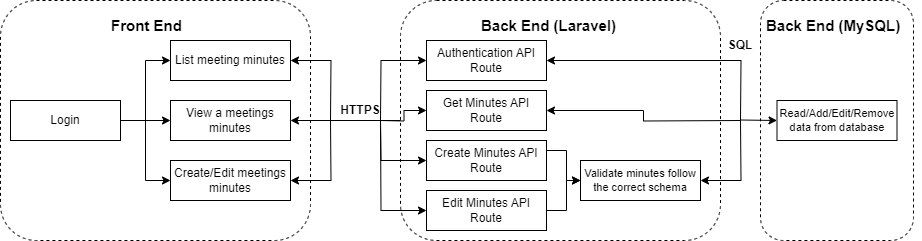
\includegraphics[width=\textwidth]{"./assets/methodology-assets/Methodology - Flow Diagram v2.drawio.png"}
\label{fig:app_design}
\end{center}
\caption{Proposed application flow.}
\end{figure}

Figure \ref{fig:app_design} show the proposed application flow. This is split in to 3 sections: Front End, Back End Data Processing (via Laravel) and Back end Data Storage (using a MySQL database). From the users perspective they will first log in, where they are then presented with 3 choices, to view all the existing minutes, create new minutes or edit existing minutes. Each of these options will take the user to a page written in React that allows them to perform that function. These pages will use an API to communicate with the back end server, using HTTPS as the transport protocol.  

The API will respond to these requests, however it may need to do some processing before responding. For example when editing the minutes of a meeting, we want to check that any votes have the correct quorum, and that will take place here. All operations will involve some reading or writing from the database, and these queries will take place using the querying language SQL. Due to the ORM provided by Laravel, less SQL code will need to be written as, this will handle a lot of the querying in an object oriented fashion. Once the data has been retrieved or written from the database, Laravel will then respond back over HTTPS with the response of the query, where React can then can then display the information in a meaningful fashion.

\section{Testing Plan}
Testing the application will be done through a series of automated and manual tests. These tests will be based around the requirements and the analysis of a governing document conducted in section \ref{sec:analyisis_governing_doc}. Both the model (via the API) and the website should be tested and from these tests it will be possible to determine to what extent the requirements have been met.

\chapter{Implementation}
\label{cha:implementation}
This chapter discusses the implementation of the application. As discussed in section \ref{sec:application_design}, this project will follow the ORM model for development and therefore, this chapter is split into 3 sections describing an overview of each: Database, API, Front End. For development this project made extensive use of Github for code management as well as Github Codespaces for a containerised development environment. 

\section{Database}
\label{sec:database}
Laravel supports 5 different types of database, however this project used Maria DB. This was chosen for two reasons: it provides better performance and its integration with Laravel.

While some of the tables and relationships were simple to implement, deciding how store the resolutions and votes was more complex. The obvious solution to this was to separate it out in to two tables: "resolutions" and "votes for resolutions". This would mean how each trustee voted could be logged individually and have a relationship between them. This however means a lot of personal data is being stored. Likewise some charities say votes should be anonymous (meaning the votes should not be stored) and the charity commission say that for other charities a show of hand should be sufficient, meaning it would be impractical to log individual votes \cite{charity_commission_making_decisions}. For these reasons this project does not log all votes and instead records the totals for them.These values are included within the meeting minutes. 

For the meeting minutes and the attendees will be modeled as JavaScript Object Notation (JSON) arrays. JSON is fairly easy to validate within Laravel and therefore, these will then be validated against a known schema when data is put into the database. As JSON arrays can be quite long, the database uses the \textit{longtext} data type within mariadb (although new versions of mariadb do now support native JSON types). The other data types have been selected such that the primary keys are all bigints, and then the database uses relationships to link them all together. The full database entity-relationship diagram can be seen in figure \ref{fig:database}


\begin{figure}[htb]
\begin{center}
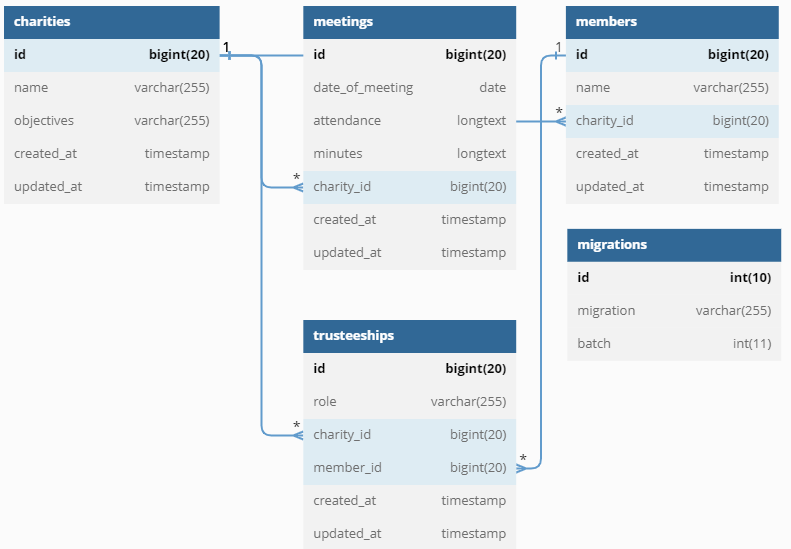
\includegraphics[width=\textwidth]{"./assets/implementation-assets/Database Diagram [Cropped].png"}
\label{fig:database}
\end{center}
\caption{Database Entity-Relationship diagram.}
\end{figure}

The migrations table seen in fig \ref{fig:database} is not used directly by the application, but instead used for version controlling the database within Laravel. It means the database migrations are stored within the Git repository and the table stores which migrations have been run on the database. 

To allow me to test the database and API the project created a series of Factories and Seeders within Laravel to populate the database. Factories create test data for the application that looks real but is actually fake. The seeder then uses these factories to create data that can be put into the database. These became particularly useful when writing unit tests as known data was in the database.


\section{Backend Processing and API}
Once the database structure was designed, the Model for the charity could be created. With Laravel each table within the database has its own model which all link together. Because of this standardisation Laravel hides the the vast majority of the functionality (primarily inputting and retrieving data from the database) in Parent classes, so the models created were relatively simple. This project had four Models (the code for which are shown in \nameref{sec:apendix_code}): Charity, Member, Trusteeship and Meeting. 

The models on their own do not create a website, they are just an abstract implementation of the concepts implemented within the database. To provide the API, Laravel requires that Controllers are used. These classes contain the functions that take in the HTTP request and use the models to gather the data from the database. This data is then passed to a Resource generator for each model, which converts the model into a standard JSON response, which is then returned back to the client. All HTTP requests have both a time and bandwidth cost for the user, so to reduce the number of API calls, this project combined some of the models together, using the relationships within the API. This meant that there were controllers for Charities (allowing charities to be viewed but also returning their trustees and members among other HTTP routes), Meetings (with HTTP routes for creating, editing and viewing them), and Members (allowing them to be viewed).

Where data was being added to the database the inputs needed to be validated. For this Laravel provides Rules that can be applied to input. These rules check if the input is expected and pass the request to the controller if it is or return an error message if not. While Laravel provides a wide array of Rules out of the box, two custom rules to validate the JSON for the meeting minutes and meeting attendees were required. These rules were where the project checks whether quorum has been met, ensures that the maximum votes is the same as the number of trustees that are present in the attendance log, and validates the JSON to ensure it is all the correct format. The code for these functions can be found in "\nameref{sec:apendix_code}". 

\section{Front End}
\label{sec:front_end}
In creating the front end it was important to have a user persona in mind to focus the development of the front end. For this the user persona Susan was created (who was not based on anyone real). She is the secretary of a small charity and therefore during meetings she is responsible for taking minutes and ensuring votes are valid. This is an impotent role in ensuring compliance of the charity. Throughout the meeting she needs to be able to create a meeting relation, edit the meeting (adding minutes and votes) and view the meeting minutes back afterwards. She may also want to view the trustees of the charity (to allow any manual registers to be taken) and any other details about the charity.

From this the sitemap of features that's Susan would use has been created and can be seen in figure \ref{fig:sitemap}. In principle however, for each of the API routes there is a page on the front end that uses and manipulates the data that the route provides. This means that there are 6 key pages that are used in the creation of meeting minutes: list all charities, list all meetings within a charity, create new meetings, view meetings and edit meetings. There are also other pages that allow users to do things such as view all of the charities members and view information about the charity. These are all functions that Susan would need to complete through the meeting.


\begin{figure}[htb]
\begin{center}
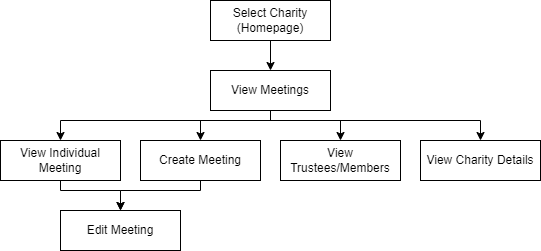
\includegraphics[width=0.85\textwidth]{"./assets/implementation-assets/Site Map v2.drawio.png"}
\end{center}
\caption{Sitemap of the website pages the user persona would follow.}
\label{fig:sitemap}
\end{figure}

Susan starts off a new trustee meeting on the home page where she is asked to select the charity that the minutes are for. From there she is able to view all of the meetings that have taken place in the charity. From here she can follow links to pages containing all of the charity's members, the charity's details and to view the minutes of a previous meeting. However, as this is a new meeting, she navigates to create a new meeting where she is presented with a form to input the date the meeting took place. From there she then is taken to the edit meeting page.

While screenshots of all the pages can be found in "\nameref{sec:apendix_screenshots}", the edit meeting page is of particular interest. It was important for users to be able to add sections (of text and different votes) into the minutes of a meeting. For this the project was able to implement a custom minute editor that allows for a user to hover over a gap between sections (or at the end of the document) where buttons are shown, to add text sections (of Markdown formatted text) or vote sections. Likewise when a user hovers over a section, a red button appears that allows them to delete the section. When there is a change to the document via one of these mechanisms and there has been no activity for 500 milliseconds, the browser auto saves the document. This is all shown in figure \ref{fig:edit_minutes_buttons}.

\begin{figure}[htb]
\begin{center}
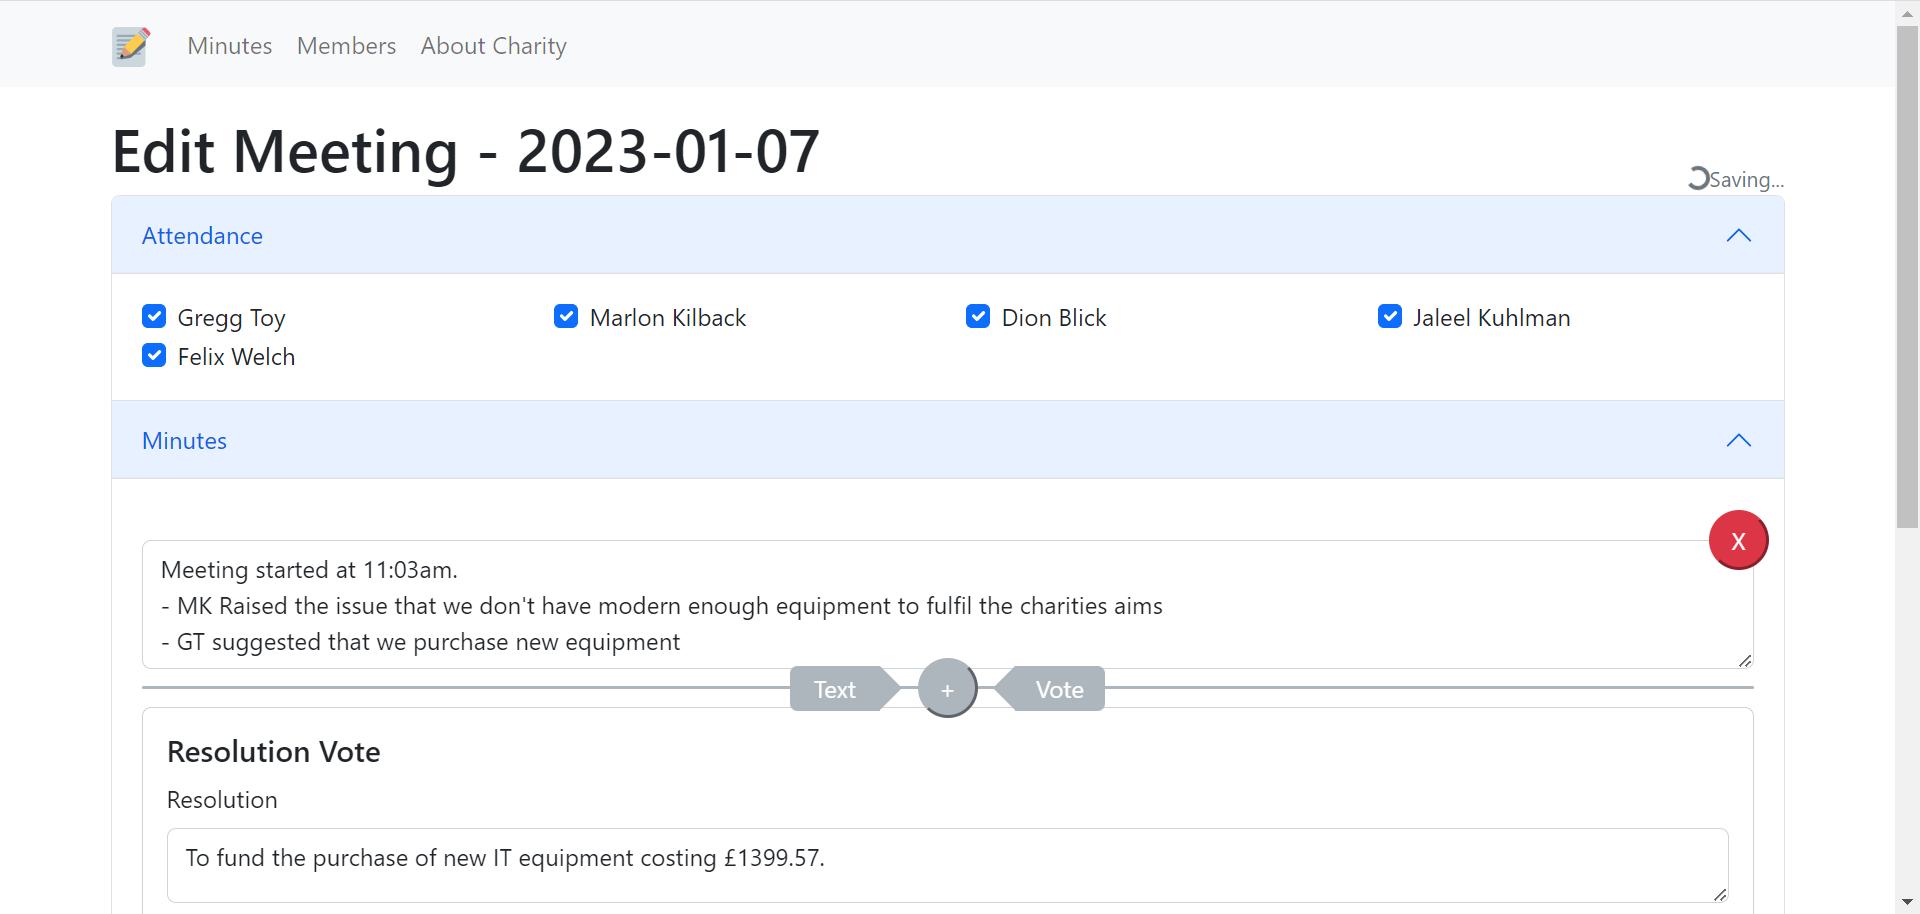
\includegraphics[width=\textwidth]{"./assets/apendix/frontend-screenshots/Minutes Edit - Buttons.png"}
\end{center}
\caption{Buttons to add and remove sections in the minutes.}
\label{fig:edit_minutes_buttons}
\end{figure}

Once the Susan has added a vote they are shown a form like in figure \ref{fig:edit_minutes_buttons} to edit it. Any errors with the vote are shown in yellow at the top, while the result is shown at the bottom. As there is an error there is no result, however if the resolution is successful this would turn green and if it failed it would go red. Any abstentions are not recorded in the form.

\begin{figure}[h]
\begin{center}
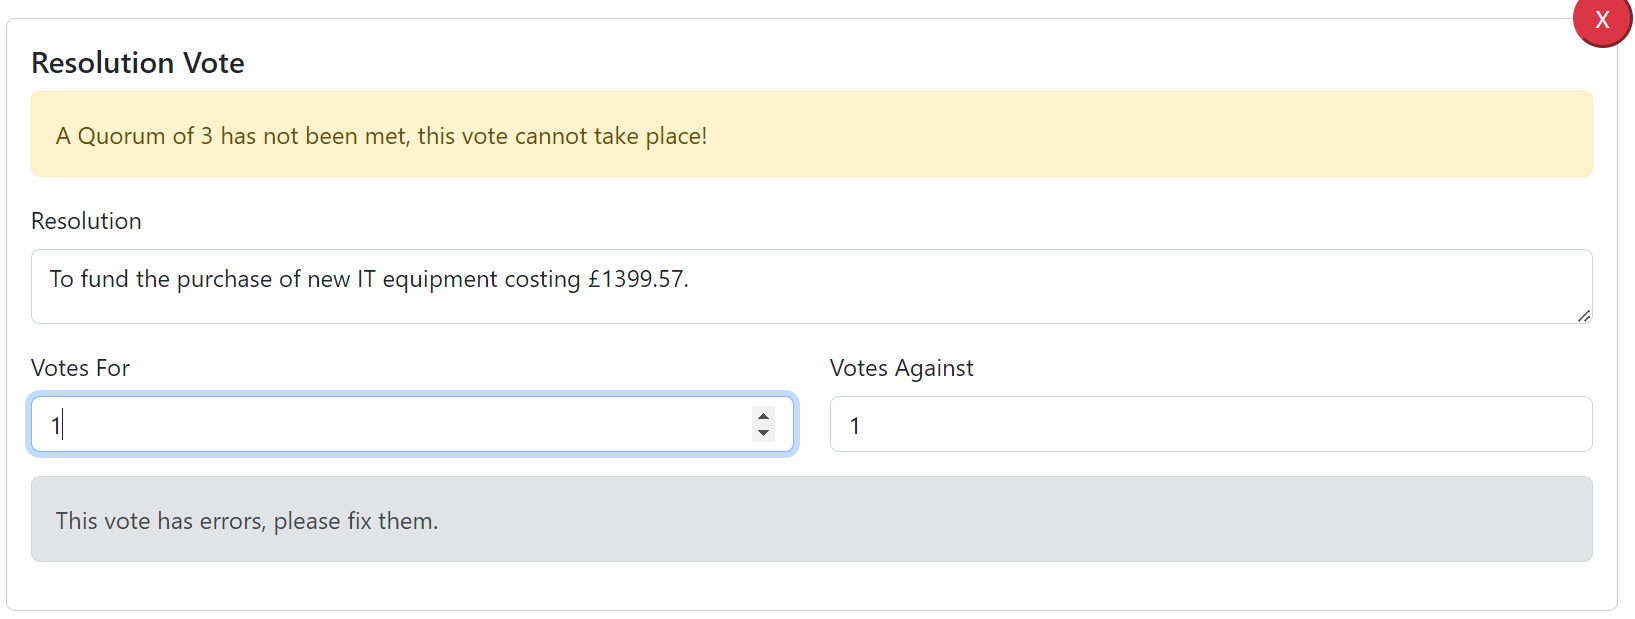
\includegraphics[width=\textwidth]{"./assets/apendix/frontend-screenshots/Minutes Edit - Errors.png"}
\end{center}
\caption{A display of the form to edit a vote with errors.}
\label{fig:edit_minutes_errors}
\end{figure}

From the edit meeting page Susan can now both minute the meeting and confirm that the votes taking place within the meeting are compliant with the governing document.

While this project could have created its own website styling for the pages, its purpose was instead to prove that you could model a charity. For this reason this project used Bootstrap \cite{bootstrap_homepage} to create most of the components (using the JS implementation \textit{react-bootstrap}\cite{react_bootstrap_2023}). Using this also had the advantage of making the project accessible by default \cite{otto_thornton_bootstrap_2021}. To allow these components to be extended there was a need for custom CSS to be injected into some of them. For this the library \textit{styled-components} was selected due to its ability to map components and styles together. Many of the pages contain links and as such a routing mechanism was needed on the front end app to allow the page to be changed; the library \textit{react-router} was used for this\cite{react-router}.




\section{Issues and Limitations}
There were some issues that arose while implementing the solution. The first of these arose while implementing the database. Maria DB unfortunately does not support the JSON column type. Other databases that Laravel supports (such as MySQL and MongoDB) do support it \cite{quackit}. The compromise here was that the JSON is stored as strings rather than as the data structure. This however means that that these columns are difficult to search using native SQL. Another issue encountered was with saving of the minutes. Initially these sent an API call updating the meeting after every single keystroke, however there were some concurrency issues with this. Sometimes the packets would not send correctly, meaning the database would be storing different data to what was displayed on the users computer. This issue was solved by having a timeout on the auto save functionality, so that it only saves once every 500 milliseconds \cite{himanshu_2021}. The final major issue that was encountered was displaying the validation errors on the vote. As you can see within figure \ref{fig:vote_validateion_code} the Laravel only allows for text failure messages to be returned to the client. This means that it is impossible to know within the JS code which section in the minutes caused the error as they will all get lumped into one. To get around this I started all the error messages with "Item <number> - " and then used the following regular expression to extract the group and message respectively: \verb|^Item ([0-9]+) - (.+)$|

Throughout the implementation there were some limitations with the solution. The first of these was how to store vote data as discussed in section \ref{sec:database}. If a trustee is deleted from the database, the JSON stored will not be updated. This means that while a vote is valid at the time, if a trustee is removed, the vote could no longer pass the validation rules. If database tables had been used in their place the references could be automatically updated without affecting previous votes. 



\chapter{Testing, Results \& Evaluation}
\label{cha:testing}

\section{Testing}
To be able to evaluate the developed application against the requirements, a series of tests were conducted to ensure the website was operating as expected. These tests were split in to two categories: Automated Unit Testing and Manual Testing. The aim of the automated testing was to ensure that the server and database components were working correctly, while the manual testing was to ensure that the user interface was working correctly. The manual testing could have been automated via tools such as Microsoft Playwright \cite{microsoft_playwright}, which would have been a more exact science, but due to time constraints this was not implemented. 



\subsection{Automated Unit Testing}
The unit testing aim was to test the server and database. To facilitate this Laravel has a unit test suit built in that allows mock API calls (with assertions about the response data), and database queries (with assertions that data has been added or manipulated in certain ways). For this Laravel builds upon the existing testing framework PHPUnit \cite{phpunit}. While the majority of the API routes had tests written for them (confirming that the route did what it claimed), the vast majority of the tests revolved around confirming the validation of a meeting was accurate. To ensure that while developing the project that functionality was not accidentally removed, a Github Action (Github's proprietary continuous integration platform) which ran the tests and posted the results (along with the code coverage) back to the repository. In total there were 20 tests achieving a total code coverage of 81.82\% of the server components as shown in "\nameref{sec:apendix_file_strictures}". These are all shown in the table \ref{table:unit_test_results}.

\begin{table}[H]
\resizebox{\textwidth}{!}{%
\begin{tabular}{|r|l|l|}
\hline
\multicolumn{1}{|l|}{\textbf{ID}} & \textbf{Description} & \textbf{Result} \\ \hline
1 & Test Charity seeder & Passed \\ \hline
2 & Test Charity api get all route & Passed \\ \hline
3 & Test Charity api get route & Passed \\ \hline
4 & Test Meeting api get returns meetings & Passed \\ \hline
5 & Test Meeting api get individual meeting & Passed \\ \hline
6 & Validate minutes text has too many keys & Passed \\ \hline
7 & Validate minutes has value key & Passed \\ \hline
8 & Validate minutes value is string & Passed \\ \hline
9 & Validate vote contains correct keys & Passed \\ \hline
10 & Validate vote resolution is string & Passed \\ \hline
11 & Validate vote votes for is int above 0 & Passed \\ \hline
12 & Validate vote votes against is int above 0 & Passed \\ \hline
13 & Validate vote total votes more than number of trustees & Passed \\ \hline
14 & Validate vote total votes more than 
attendance & Passed \\ \hline
15 & Validate vote present trustees more than 
quorum of two thirds trustees & Passed \\ \hline
16 & Validate vote present trustees more than 
quorum of two & Passed \\ \hline
17 & Validate attendance charity does not exist & Passed \\ \hline
18 & Validate attendance trustee does not exist & Passed \\ \hline
19 & Validate attendance trustee is not part of charity & Passed \\ \hline
20 & Member api get route & Passed \\ \hline
\end{tabular}%
}
\caption{Unit test results}
\label{table:unit_test_results}
\end{table}





\subsection{Manual Testing}
The manual tests primarily cover testing UI components that could not be tested via the unit tests. Some of these are fairly concrete (such as checking a page exists) however, others of them are more subjective, such as seeing if something is in an easy to understand format. This is an issue with this method of testing and a future project could survey potential users to see what they think of the elements being tested. That being said some of the tests failed, however this was mainly because those features were not implemented. The tests ran and their results, along with a brief description on how to run them, are shown in \ref{table:manual_test_results}


\begin{landscape}
\begin{table}[]
\resizebox{\textheight}{!}{%
\begin{tabular}{|r|l|l|l|l|l|l|}
\hline
\multicolumn{1}{|l|}{\textbf{ID}} & \textbf{Description} & \textbf{Requirement No} & \textbf{Steps} & \textbf{Expected Result} & \textbf{Passed/Fail} & \textbf{Comments} \\ \hline
1 & Is the code commented & 1.7 & Pick 5 random files and is see if the code has been commented. & The code should be commented & Passed &  \\ \hline
2 & \begin{tabular}[c]{@{}l@{}}There is a page that allows you\\ to login\end{tabular} & 1.8 & Open the website, this should be the first page that is displayed & A login screen should appear & Failed & The feature was not implemented \\ \hline
3 & \begin{tabular}[c]{@{}l@{}}There is a page that allows you\\ to select the charity to view\end{tabular} & 1.8 & Use the application and see if the page exists in a logical place. & \begin{tabular}[c]{@{}l@{}}A page with a table containing all the charities\\  in the database\end{tabular} & Passed &  \\ \hline
4 & \begin{tabular}[c]{@{}l@{}}There is a page that allows you \\ to select which meeting to view\end{tabular} & 1.6, 1.8 & Use the application and see if the page exists in a logical place. & \begin{tabular}[c]{@{}l@{}}A page with a table containing all the meetings \\ a charity has held\end{tabular} & Passed &  \\ \hline
5 & \begin{tabular}[c]{@{}l@{}}There is a page that allows you\\ to create new meetings\end{tabular} & 1.8 & Use the application and see if the page exists in a logical place. & \begin{tabular}[c]{@{}l@{}}A page containing a form with fields to create \\ a new meeting\end{tabular} & Passed &  \\ \hline
6 & \begin{tabular}[c]{@{}l@{}}There is a page that allows you\\  to edit a meeting\end{tabular} & 1.8 & Use the application and see if the page exists in a logical place. & \begin{tabular}[c]{@{}l@{}}A page containing a form that allows you to\\  edit a meeting\end{tabular} & Passed &  \\ \hline
6.1 & \begin{tabular}[c]{@{}l@{}}When editing a meeting, the \\ minutes and votes are displayed\\ in an easy to understand format\end{tabular} & 1.9 & Create a new meeting & \begin{tabular}[c]{@{}l@{}}It should be easy to create a vote, text and \\ track the attendance of the meeting.\end{tabular} & Passed &  \\ \hline
6.2 & \begin{tabular}[c]{@{}l@{}}Any errors with a vote are\\ displayed to the user\end{tabular} & 1.9 & \begin{tabular}[c]{@{}l@{}}Create a new meeting, and set the number of votes to a number\\  above the number of trustees in a charity.\end{tabular} & A error message is displayed to the user. & Passed &  \\ \hline
6.3 & \begin{tabular}[c]{@{}l@{}}When editing a meeting is \\ the markdown formatted.\end{tabular} & 1.5 & \begin{tabular}[c]{@{}l@{}}Create a new meeting, input markdown into the text or \\ resolution fields\end{tabular} & \begin{tabular}[c]{@{}l@{}}The markdown should be formatted even \\ while editing the form\end{tabular} & Failed & \begin{tabular}[c]{@{}l@{}}There is only a plain text view \\ while editing - it is only rendered \\ while viewing the minutes.\end{tabular} \\ \hline
7 & \begin{tabular}[c]{@{}l@{}}There is a page that allows \\ you to view a meeting\end{tabular} & 1.6, 1.8 & Use the application and see if the page exists in a logical place. & \begin{tabular}[c]{@{}l@{}}A page with a table containing the attendance \\ and minutes of the given meeting\end{tabular} & Passed &  \\ \hline
7.1 & \begin{tabular}[c]{@{}l@{}}Can user input markdown \\ into a text section of the minutes\end{tabular} & 1.5 & \begin{tabular}[c]{@{}l@{}}Create a new meeting, then input raw markdown into a text \\ section in the minutes, then view those minutes.\end{tabular} & The markdown should be formatted & Passed &  \\ \hline
7.2 & \begin{tabular}[c]{@{}l@{}}Can user input markdown \\ into a resolution section of the\\ minutes\end{tabular} & 1.5 & \begin{tabular}[c]{@{}l@{}}Create a new meeting, then input raw markdown into a \\ resolution in a votes section in the minutes, then view\\ those minutes.\end{tabular} & \begin{tabular}[c]{@{}l@{}}The resolution should be formatted \\ as markdown\end{tabular} & Passed &  \\ \hline
7.3 & \begin{tabular}[c]{@{}l@{}}When viewing a meeting, the \\ minutes and votes are displayed\\ in an easy to understand format\end{tabular} & 1.9 & Open a meeting & \begin{tabular}[c]{@{}l@{}}The page should track downwards with attendance\\ at the top and deadening displaying the \\ information about the meeting.\end{tabular} & Passed &  \\ \hline
7.4 & \begin{tabular}[c]{@{}l@{}}The website should work with \\ a screen reader\end{tabular} & 2.6 & Open a meeting and get a screen reader to read the minutes out. & \begin{tabular}[c]{@{}l@{}}The minutes should be read out in the correct \\ order, and all the information should be given.\end{tabular} & Passed & \begin{tabular}[c]{@{}l@{}}Using "texthelp Read\&Write" \\ screen reader software\end{tabular} \\ \hline
8 & \begin{tabular}[c]{@{}l@{}}There is a page that allows you\\  to see all members\end{tabular} & 1.8 & Use the application and see if the page exists in a logical place. & \begin{tabular}[c]{@{}l@{}}A page with a table containing all the members\\  that are part of the given charity\end{tabular} & Passed & Combined with trustees \\ \hline
9 & \begin{tabular}[c]{@{}l@{}}There is a page that allows you\\ to see all Trustees\end{tabular} & 1.8 & Use the application and see if the page exists in a logical place. & \begin{tabular}[c]{@{}l@{}}A page with a table containing all the trustees \\ that are part of the given charity\end{tabular} & Passed & Combined with members \\ \hline
\end{tabular}%
}
\caption{Manual Test Results}
\label{table:manual_test_results}
\end{table}
\end{landscape}



\section{Evaluation Against Success Criteria}
In addition to the tests carried out, an in depth evaluation against the requirements was completed. Due to time constraints some functionality has not been implemented (or was only partially implemented) in the project. A full table of all the requirements and their ratings can be seen in table \ref{table:requirements_evaluation}.



% Please add the following required packages to your document preamble:
% \usepackage{graphicx}
\begin{table}[]
\resizebox{\textwidth}{!}{%
\begin{tabular}{|l|l|r|l|}
\hline
\textbf{ID} & \textbf{Requirement} & \multicolumn{1}{l|}{\textbf{Rating}} & \textbf{Comments} \\ \hline
1.1 & \begin{tabular}[c]{@{}l@{}}The application must have a database \\ containing charity meetings, the \\ minutes, votes, and trustees\end{tabular} & 2 & \begin{tabular}[c]{@{}l@{}}The database contains all of this information \\ over the various tables.\end{tabular} \\ \hline
1.2 & \begin{tabular}[c]{@{}l@{}}The application must take in the\\  minutes of a meeting and return \\ confirm that they are valid\end{tabular} & 3 & \begin{tabular}[c]{@{}l@{}}The application validates the user input \\ before it is saved to the database to \\ ensure the meeting is valid.\end{tabular} \\ \hline
1.3 & \begin{tabular}[c]{@{}l@{}}A data structure should be created \\ for a meeting that can be easily\\ validated\end{tabular} & 3 & \begin{tabular}[c]{@{}l@{}}A JSON data structure was selected and \\ was validate using Laravel's Rules.\end{tabular} \\ \hline
1.4 & \begin{tabular}[c]{@{}l@{}}A valid meeting should ensure that\\  quorum is met for all votes\end{tabular} & 3 & \begin{tabular}[c]{@{}l@{}}The validator checks this a returns an error \\ if it is not met.\end{tabular} \\ \hline
1.4.1 & \begin{tabular}[c]{@{}l@{}}If it is a constitutional amendment\\  then at least 75\% of members \\ should vote for it to pass\end{tabular} & 0 & \begin{tabular}[c]{@{}l@{}}This was not implemented, however future projects\\ could extend the current implementation quite \\ easily to add this.\end{tabular} \\ \hline
1.4.2 & \begin{tabular}[c]{@{}l@{}}If it is a resolution is up for vote the\\ for it to pass it must have at least \\  two charity trustees, or the number \\ nearest to one third of the total number \\ of charity trustees, whichever is higher \\ vote for it to pass\end{tabular} & 3 & \begin{tabular}[c]{@{}l@{}}The validator checks the number of trustees\\ and sets the quorum threshold accordingly.\end{tabular} \\ \hline
1.5 & \begin{tabular}[c]{@{}l@{}}A user should be able to input \\ markdown as plain text input for the \\ minutes of a meeting\end{tabular} & 2 & \begin{tabular}[c]{@{}l@{}}A user can use markdown and it is formatted \\ correctly when the information is displayed, however\\ there is no indication of this on the front end, nor is it \\ particularly user friendly for people that do not\\ already know markdown.\end{tabular} \\ \hline
1.6 & \begin{tabular}[c]{@{}l@{}}A user should be able to view\\  meetings afterwards\end{tabular} & 3 & \begin{tabular}[c]{@{}l@{}}There are both API routes and pages on the \\ front end for displaying a meeting.\end{tabular} \\ \hline
1.7 & \begin{tabular}[c]{@{}l@{}}Code should be commented for \\ future maintainability\end{tabular} & 3 & \begin{tabular}[c]{@{}l@{}}All code was commented with single-line comments\\ explaining code within comments and comments \\ following the PHPDoc standard were used to define \\ functions and classes.\end{tabular} \\ \hline
1.8 & The application should be easy to use & 2 & \begin{tabular}[c]{@{}l@{}}By using a standard framework, Bootstrap, the\\ user interface looks and behaves like any other \\ website. Further surveys would be needed \\ however to confirm what users think of it.\end{tabular} \\ \hline
1.9 & \begin{tabular}[c]{@{}l@{}}The application should display \\ minutes and votes in an easy to \\ understand format\end{tabular} & 3 & \begin{tabular}[c]{@{}l@{}}It is clear when editing and viewing meeting\\  minutes where there are votes, what was being \\ voted on and, any other business that was \\ conducted in the meeting.\end{tabular} \\ \hline
2.1 & \begin{tabular}[c]{@{}l@{}}The application should allow for \\ the election of new trustees to be\\  included in the minutes of a meeting\end{tabular} & 1 & \begin{tabular}[c]{@{}l@{}}The current implementation could allow for this \\ assuming a user uses the resolution as a vote (as \\ the quorum would be the same), however it would\\ be rather confusing to do this as the labels would \\ be wrong.\end{tabular} \\ \hline
2.2 & \begin{tabular}[c]{@{}l@{}}The application should allow trustee\\  resignations to be included in \\ the minutes of a meeting\end{tabular} & 1 & \begin{tabular}[c]{@{}l@{}}This could be minuted via text, however \\ currently there is no mechanism to remove \\ the trustee from the database, therefore this\\ would need extending.\end{tabular} \\ \hline
2.3 & \begin{tabular}[c]{@{}l@{}}Each trustee has their own user\\ account and can log in to \\ view minutes of the meetings\end{tabular} & 0 & This functionality has not been included. \\ \hline
2.4 & \begin{tabular}[c]{@{}l@{}}The application should have \\ separate rules for general \\ meetings and trustee meetings\end{tabular} & 0 & This functionality has not been included. \\ \hline
2.5 & \begin{tabular}[c]{@{}l@{}}The application should run on\\  the web\end{tabular} & 3 & \begin{tabular}[c]{@{}l@{}}The application does run on the web, using \\ PHP on the back end and Javascript on \\ the front end.\end{tabular} \\ \hline
2.6 & \begin{tabular}[c]{@{}l@{}}The application should be screen \\ reader compliant for people \\ with disabilities\end{tabular} & 2 & \begin{tabular}[c]{@{}l@{}}By using bootstrap the vast majority of the \\ components are screen reader compliant \\ however a few bits need improvement\end{tabular} \\ \hline
3.1 & \begin{tabular}[c]{@{}l@{}}Web sockets should be used so\\ that multiple users can edit the same \\ meeting at once\end{tabular} & 0 & This functionality has not been included. \\ \hline
3.2 & \begin{tabular}[c]{@{}l@{}}The application should support \\ accounts for non-voting members\end{tabular} & 2 & \begin{tabular}[c]{@{}l@{}}Non voting members are included within \\ the database (as they are members without\\ a trustee relationship), however as \\ requirement 2.3 has not been implemented the\\ members do not have a password to login.\end{tabular} \\ \hline

\multicolumn{4}{l}{} \\ \hline
\multicolumn{4}{|l|}{Key for Ratings: 0 = Not Met, 1 = Somewhat Met, 2 = Mostly Met, 3 = Completely Met} \\ \hline

\end{tabular}%
}
\label{table:requirements_evaluation}

\caption{Evaluation against the requirements} 
\end{table}



\section{Future Work and Developments}
Throughout this project there have been various points where it would benefit to have further investigation. The next logical step to this project would be to conduct research into charity trustees and members via questionnaires and see if the tool in its current state would solve the issues that they are facing. While this tool did create its own user persona, Susan (in section \ref{sec:front_end}), it would be better to base this persona on a real person. Some form of usability study could also be conducted to ensure the front end side of the tool is appropriate for the targeted demographic. This should confirm that the tool is actually helping anyone taking meeting minutes and not hindering them.  

The next big development in this area would be an attempt to create a more generic tool. As discussed throughout chapter \ref{cha:methodology}, this tool focused around creating a model of one type of charity and governing document (a CIO using the Charity Commission's example documents). While the rules surrounding membership and general meeting voting vary from governing document to governing document, the quite defined rules prescribed by the Charity Commission means that this tool would be a good starting point for that development. 

That being said, an interesting development would be to look further into the discussions of section \ref{sec:database}. There are clearly disadvantages to storing the minutes and attendance of a meeting as a JSON array, especially if the system was scaled to be large enough for the numbers of charities in the UK. Ensuring database integrity within this would however be quite complex, especially if multiple people were viewing (or editing) a meeting at once. 


\chapter{Conclusion}
\label{cha:conclusion}
Trustees are expected to follow huge numbers of rules prescribed by both the law and the governing document of a charity. This research has produced a website application which can help trustees ensure that their meetings are compliant with these rules, while in the process showing that it is possible to model a charity. When trustees make mistakes and the charity commission steps in to investigate, it is clear that the minutes of the trustee meetings are of utmost importance as they show an  accurate record of the trustees decision making process. The application supports trustees in creating these minutes while showing that they can be checked for any compliance issues. With over 700,000 trustees in England and Wales running over 168,000 charities the potential impact of this research is huge.

The success provided by the project also hides some of the drawbacks. The focus on the example governing document of a Charitable Incorporated Organisation means that the findings cannot be applied to the charity sector as a whole. Likewise the method used to store attendance and minutes (via JSON) in charity meetings is not saleable to large numbers of charities. 

This research's biggest contribution is that it has shown that every action trustees take in meetings and through charity operations, affect the compliance of a charity. These decisions form a discrete system of states, that can be modelled within both an object orientated programming language, and stored for future use within a database. 

Despite any drawbacks, this project has achieved its aims by showing that it is possible to model a charity and provide an interface for that.


\chapter{Appendix}
\label{cha:apendix}

\section{Appendix 1: Summary of Governing Document Clauses}
\label{sec:apendix_1_gov_doc_sumary}

\begin{longtable}{|p{0.15\textwidth}|p{0.85\textwidth}|}
  \hline
  \textbf{Clause No.} & \textbf{What the clause does} \\\hline
  \endfirsthead
    %
    \endhead
    %
  Clause 1 & 
          Defines the name of Charity \\\hline
  Clause 2 & 
          Defines that the charity is in England and wales \\\hline
  Clause 3 & 
          Defines the main objectives of the charity \\\hline
  Clause 4 & 
          Defines the fact that the charity can borrow money, buy or take on leases for land/equipment, sell or lease land/equipment, employ staff, and invest funds. \\\hline
  Clause 5 & 
          States that trustees can be reimbursed by the charity, and with the exceptions of insurance, a trustee must not benefit financially from the charity \\\hline
  Clause 6 & 
          States that a trustee (or person connected to the trustee) must not buy or sell anything to or from the charity and that a trustee can lend money to the charity but may not charge interest more than the bank of england rate. There are certain conditions where a trustee can rent property or supply goods to the charity if certain conditions are met (including that the reasons for this are included in the minutes). \\\hline
  Clause 7 & 
          States that trustees must declare conflict of interest \\\hline
  Clause 8 & 
          Defines what should happen to assets and debt in the event the charity stops functioning. The example document provides two options for this: the trustees have no liability, or the trustees are liable up to a certain amount of money. \\\hline
  Clause 9 & 
          Defines how the trustees should operate. 

Part 1 says that trustees should act properly and use responsible care and skill.

Part 2 defines the eligibility of trustees:
A trustee must be neutral

Must be 16 or older

Must not be disqualified under charities act

Accepts the office willingly

One of the trustees must be over 18


Part 3 defines how many trustees there are, and provides 4 options for this: At least 3, A maximum number, any number and (more than a given number and less than a given number).

Clause 4 defines the first 3 trustees and how long their term is. \\\hline
  Clause 10 & 
          This clause defines how trustees are appointed. The model document provides two ways of doing:
The first is the existing trustees appoint new ones

The second way allows for existing trustees to appoint new ones, trustees to be ex-officio (i.e. the head teacher of a school automatically becomes a trustee of a charity run by that school) and trustees can be nominated by a set group of people. \\\hline
  Clause 11 & 
          This clause says that trustees should get a copy of the constitution, a copy of the accounts and a copy of the last annual report upon their appointment. \\\hline
  Clause 12 & 
          Defines that a trustee no longer holds office if they:
Resign in writing

Are absent without permission for all meetings in a 6 month period

Dies

A medical practitioner in writing informs the charity they are physically or mentally incapable of acting as trustee

Disqualified as a trustee

It also defines that a trustee can be eligible for for reappointment. \\\hline
  Clause 13 & 
          This clause defines how decisions by trustees should be taken; either at meeting of the trustees or in writing (or electric form) where the documents provided to the trustees include the resolution and the signatures on the response are verified. \\\hline
  Clause 14 & 
          States that trustees are allowed to delegate their powers, but they are ultimately responsible for the conduct of the delegate. \\\hline
  Clause 15 & 
          This clause defines how a trustee meeting should be run. Sub section one says that any trustee can call a meeting in the agreed way. Sub section two says that the trustee may appoint someone to chair the meeting and that if they are not present then a temporary one should be nominated for that meeting. Sub section 3 says that decisions must have a quorum which is two charity trustees, or the number nearest to one third of the total number of charity trustees whichever is grater and that if a trustee is not entitled to vote, they should not be counted. Subsection 4 states that a meeting can be held online if agreed by the trustees. \\\hline
  Clause 16 & 
          Defines that the only people that can be members are the trustees. \\\hline
  Clause 17 & 
          This provision is optional in the model document, however if enabled it allows trustees to create a form of non voting membership for the charity, and allows trustees to form the rights (for example the Scout association has a board of trustees, along with members but the members cannot vote). \\\hline
  Clause 18 & 
          This clause states that voting members (in this case just the trustees) must vote for all decisions relating to
Amendments to the constitution

Amalgamation with another charity

The dissolution of the charity

This clause also says that these decisions should be made at a general meeting or in writing and that 75\% of voting members must vote for all three. \\\hline
  Clause 19 & 
          This clause defines how general meetings of all members should be run. Sub section one says that charitee trustees can call a meeting at any time to allow for members to vote on a resolution as defined in clause 18. Sub section 2 states that at least 14 days notice must be given and evidence must be gathered (via email or evidence of postage) that notice was sent. Sub section 3 says that clause 15 of document governs how the meeting should be run and that there should be an electronic means to participate in the meeting. \\\hline
  Clause 20 & 
          States that if a trustee is disqualified, has retired, or was not entitled to a vote (i.e. they have a conflict of interest) then their vote in any matters should be discounted. \\\hline
  Clause 21 & 
          States that the charity should execute documents by either signing them or affixing a seal (if it has one). \\\hline
  Clause 22 & 
          States the charity must provide a hard copy of any document sent to members within 21 and that it should provide information to the charity commission on request. \\\hline
  Clause 23 & 
          States the charity must keep a register of membership and of its trustees \\\hline
  Clause 24 & 
          Defines the rules surrounding minutes, they must contain a record of:
Appointments of officers 

Proceedings of general meetings

Proceedings of charity trustees including:

who was present

Decisions made

Rationale for decisions

Decisions made by the trustees not in a formal meeting. \\\hline
  Clause 25 & 
          States that the charity must keep accounts in accordance with the charities act 2011, and that the charity must inform the charity commission if there is a change with their accounting practices. \\\hline
  Clause 26 & 
          Defines that trustees can create bylaws and enforce them. They must make these rules available on request. \\\hline
  Clause 27 & 
          Defines that disputes must be handled with good faith mediation before litigation is used. \\\hline
  Clause 28 & 
          Defines that the constitution is amended only if all members write to agree or if a resolution is passed by a 75\% majority at a general meeting (as defined in clause 19). The clause then says an updated constitution must be sent to the charity commission within 15 days. \\\hline
  Clause 29 & 
          This clause says that for the charity to be dissolved it must either put to a vote the membership (which is just the trustees) with at least two weeks' notice and to pass with at least 75\% of the votes or a resolution that is in writing and agreed to by all members. The clause then defines how the assets should be dissolved, and how the charity commission should be informed. \\\hline
  Clause 30 & 
          Defines the legal terms used throughout the document. \\\hline

\caption{ Analysis of a model governing document. } \\
\end{longtable}

\newpage
\section{Appendix 2: Code}
\label{sec:apendix_code}
\subsection{Models}


\begin{figure}[H]
\begin{center}
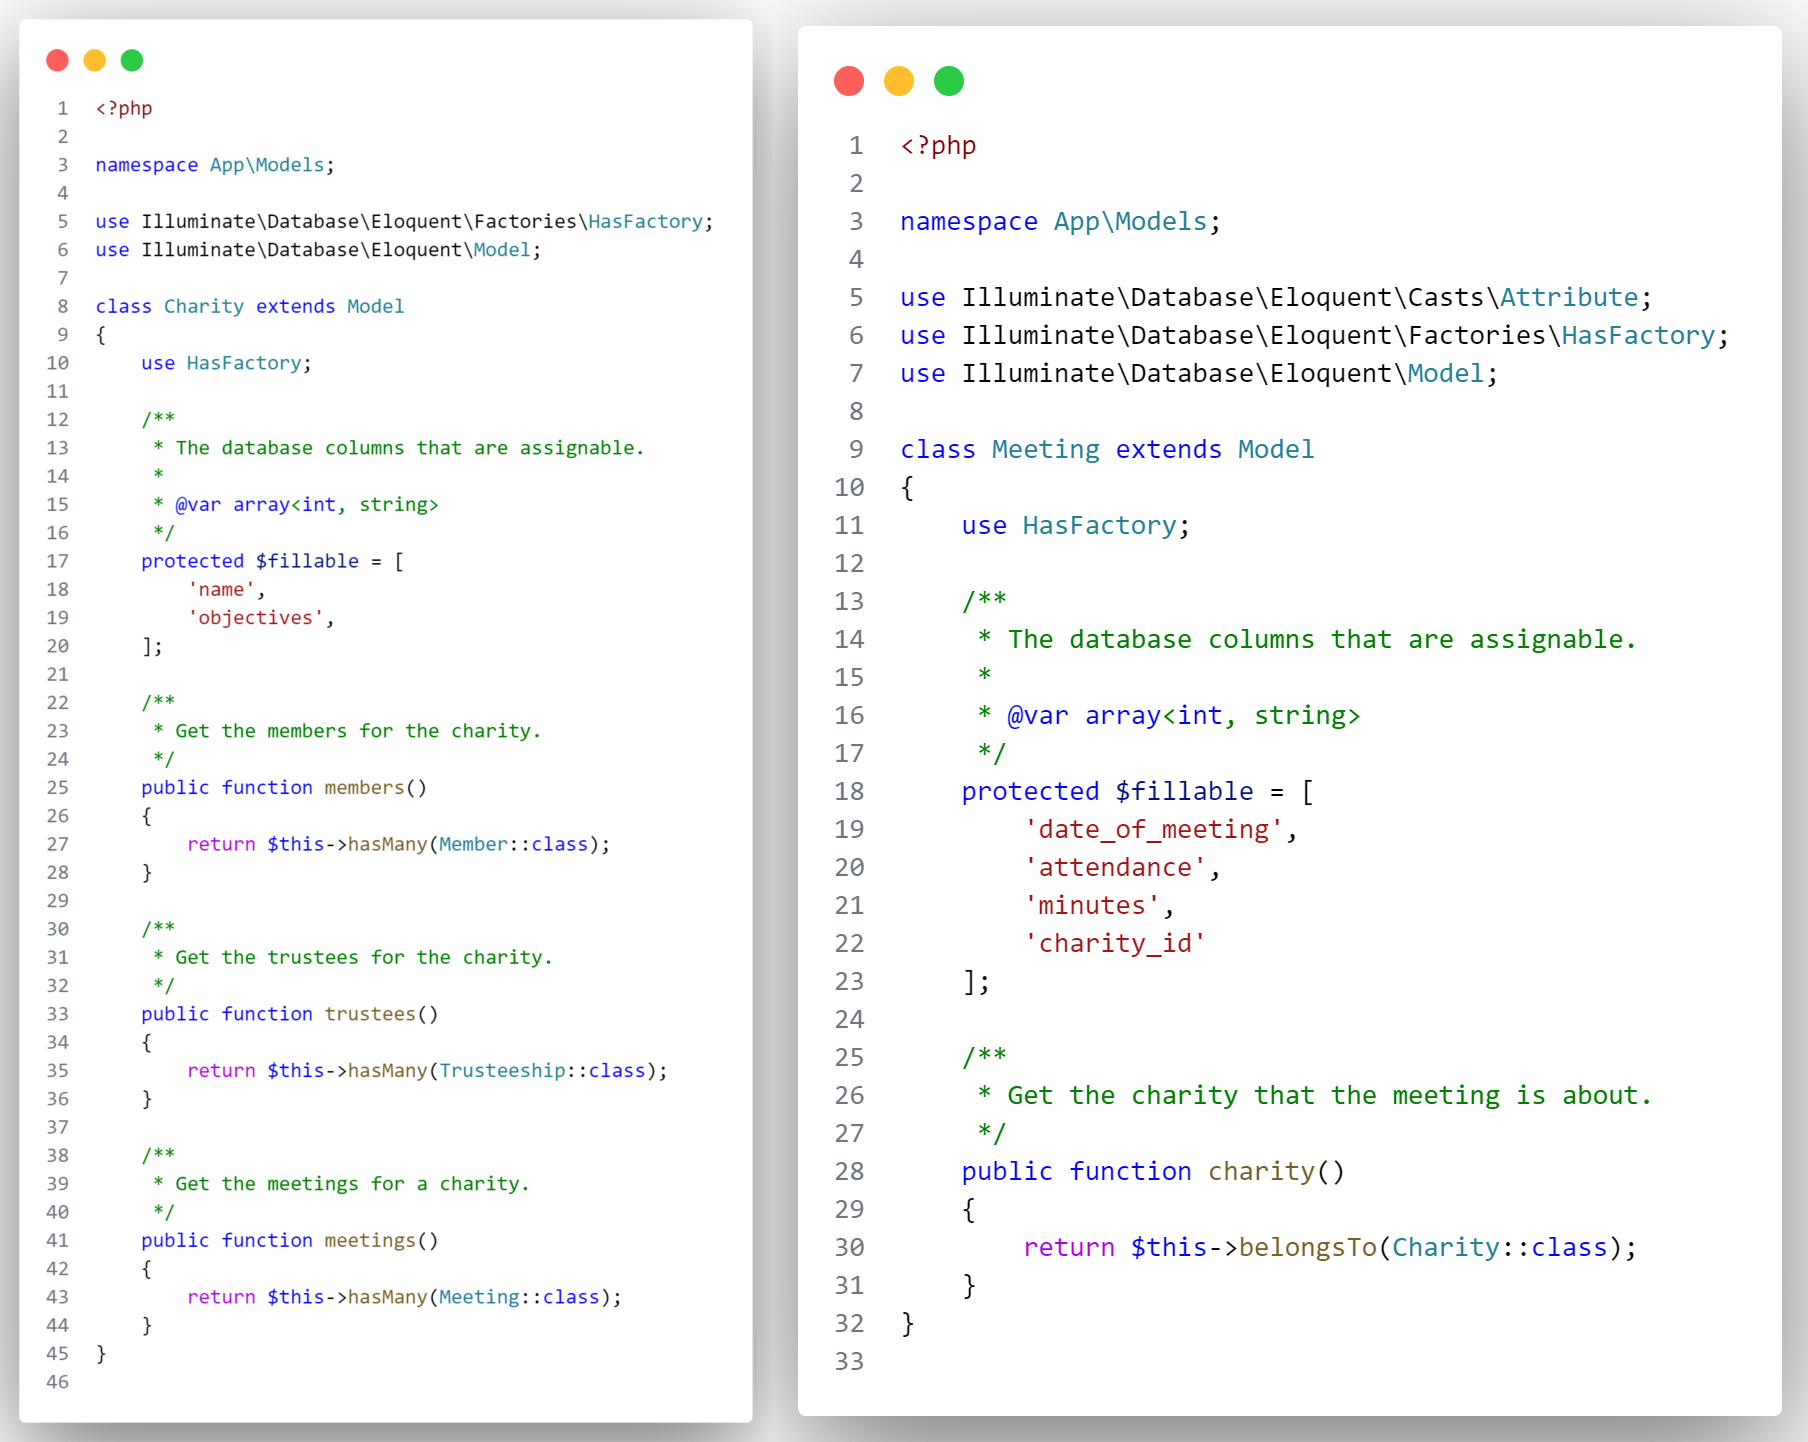
\includegraphics[width=1\textwidth]{"./assets/apendix/model-code-screenshots/Charity and Meeting Combined.png"}
\end{center}
\caption{The ORM Model for the Charity (left) and a Meeting (right).}
\end{figure}

\begin{figure}[H]
\begin{center}
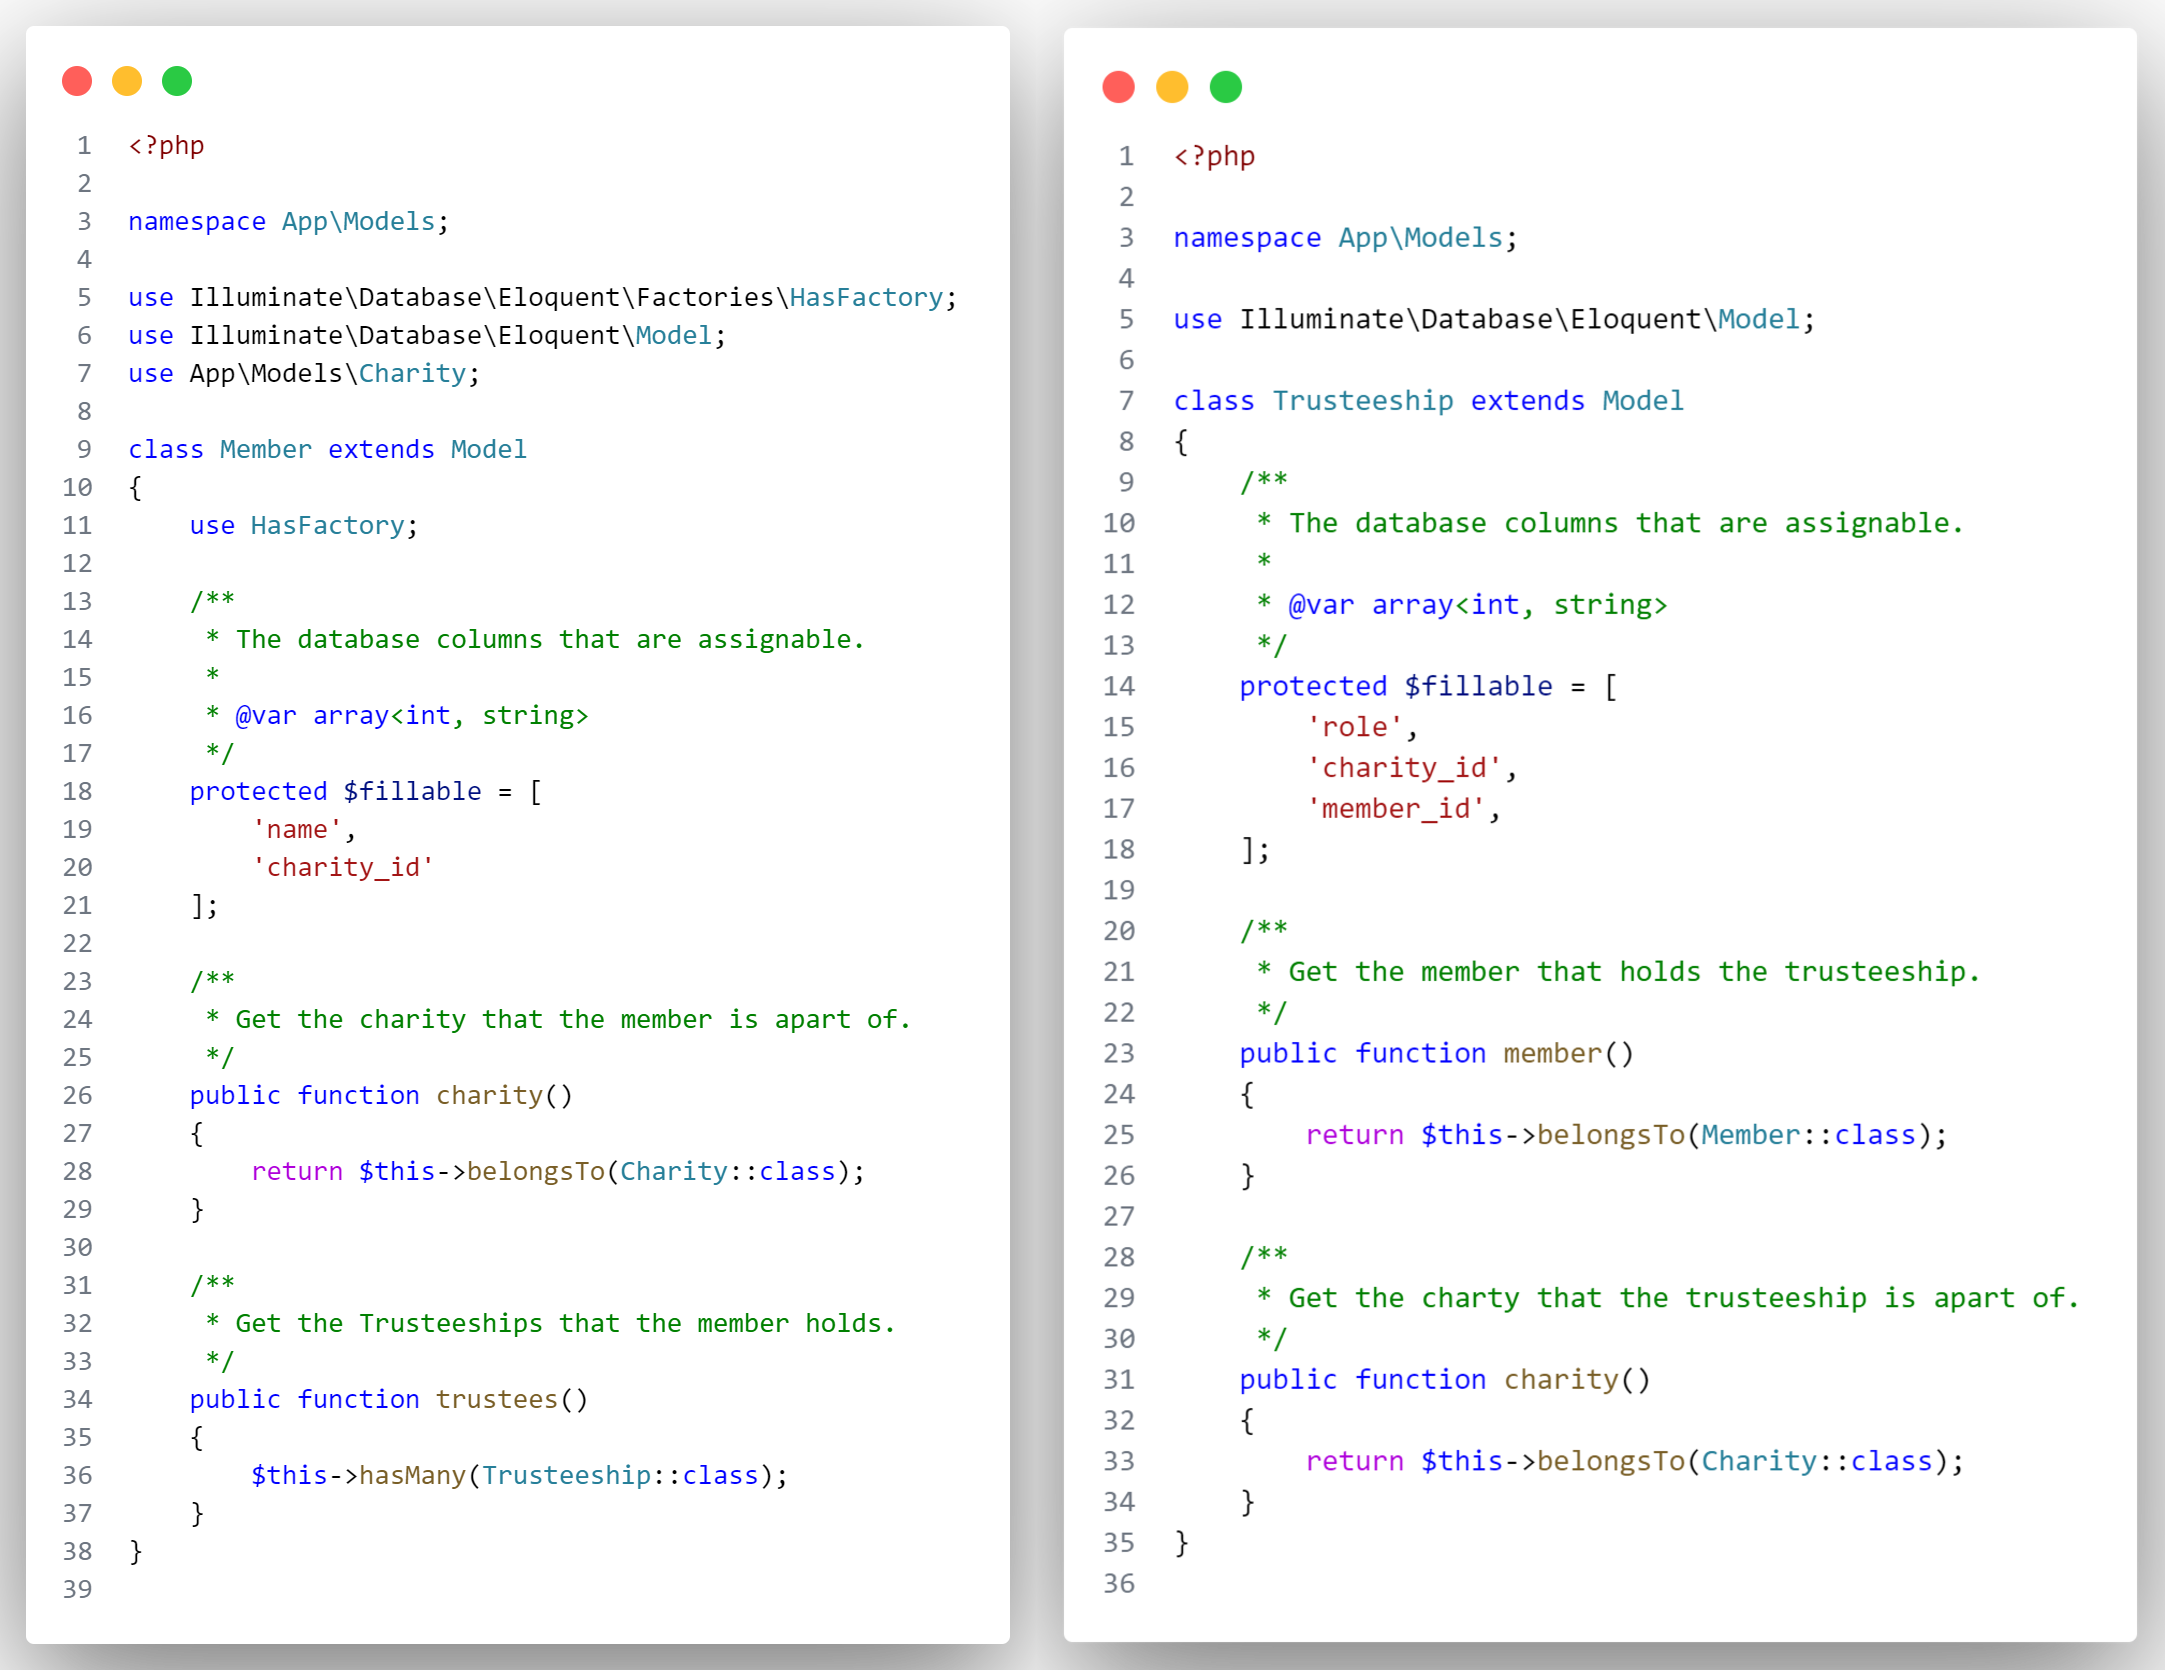
\includegraphics[width=0.9\textwidth]{"./assets/apendix/model-code-screenshots/Member and Trusteeship Combined.png"}
\end{center}
\caption{The ORM Model for a Member (left) and a Trusteeship (right).}
\end{figure}


\subsection{Validation Rules}

\begin{figure}[htb]
\begin{center}
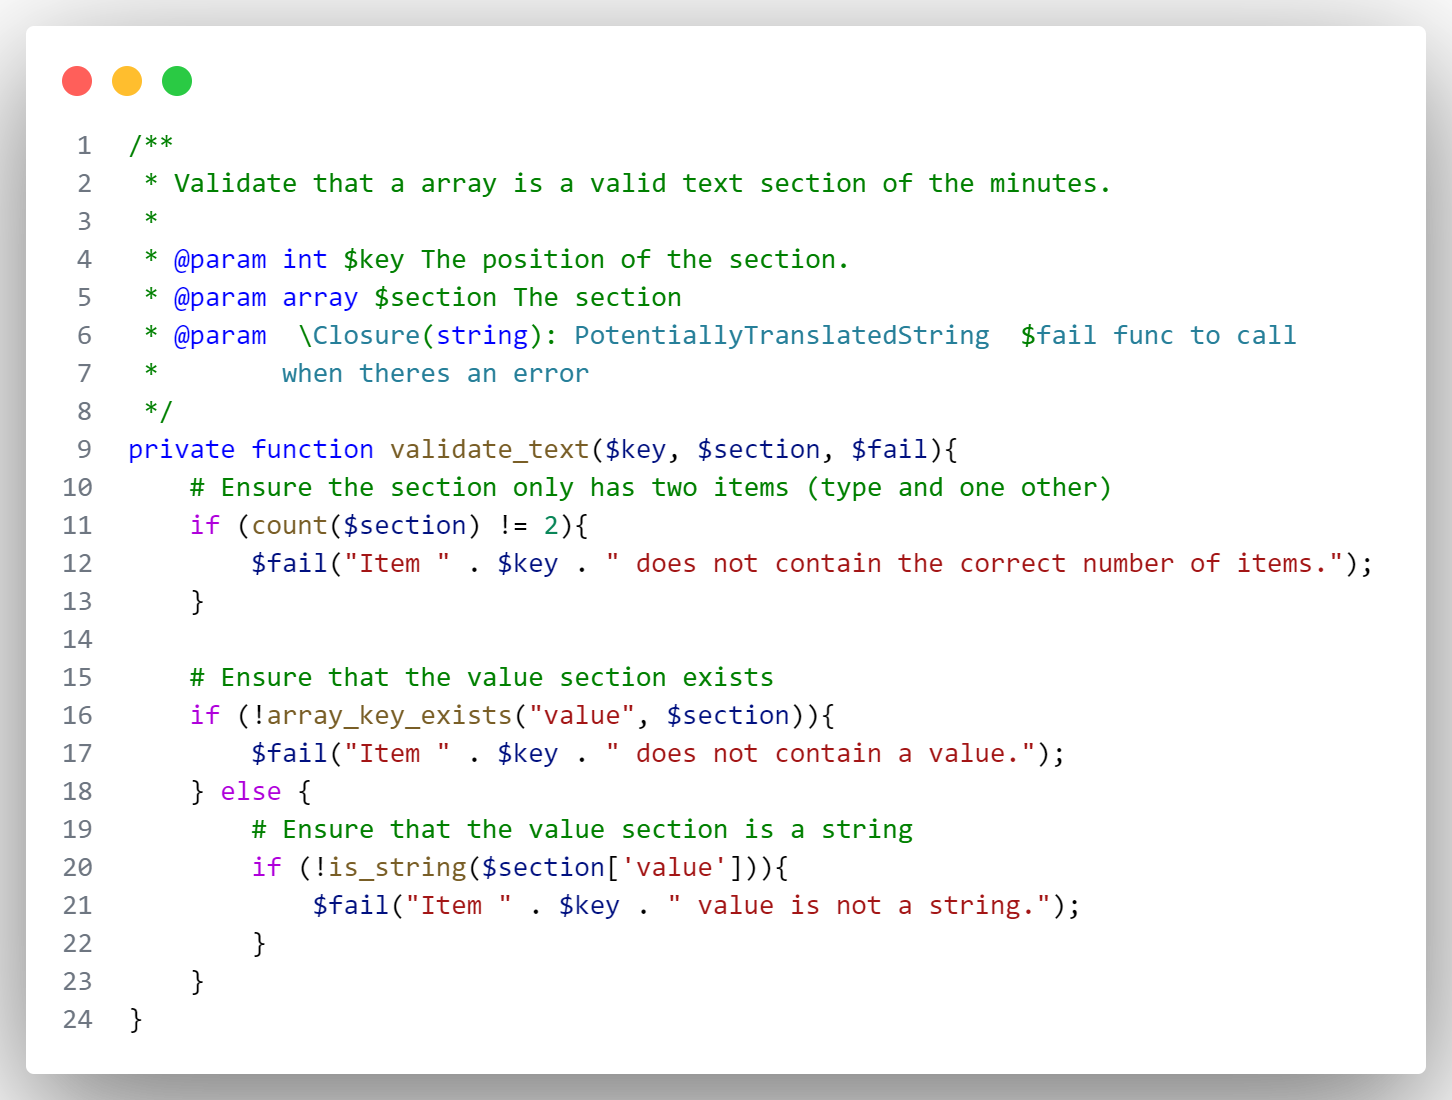
\includegraphics[width=0.715\textwidth]{"./assets/apendix/rules-code-screenshots/Minutes - Text.png"}
\end{center}
\caption{Sub function of the Minutes validation rules, validating a text section.}
\end{figure}

\begin{figure}[H]
\begin{center}
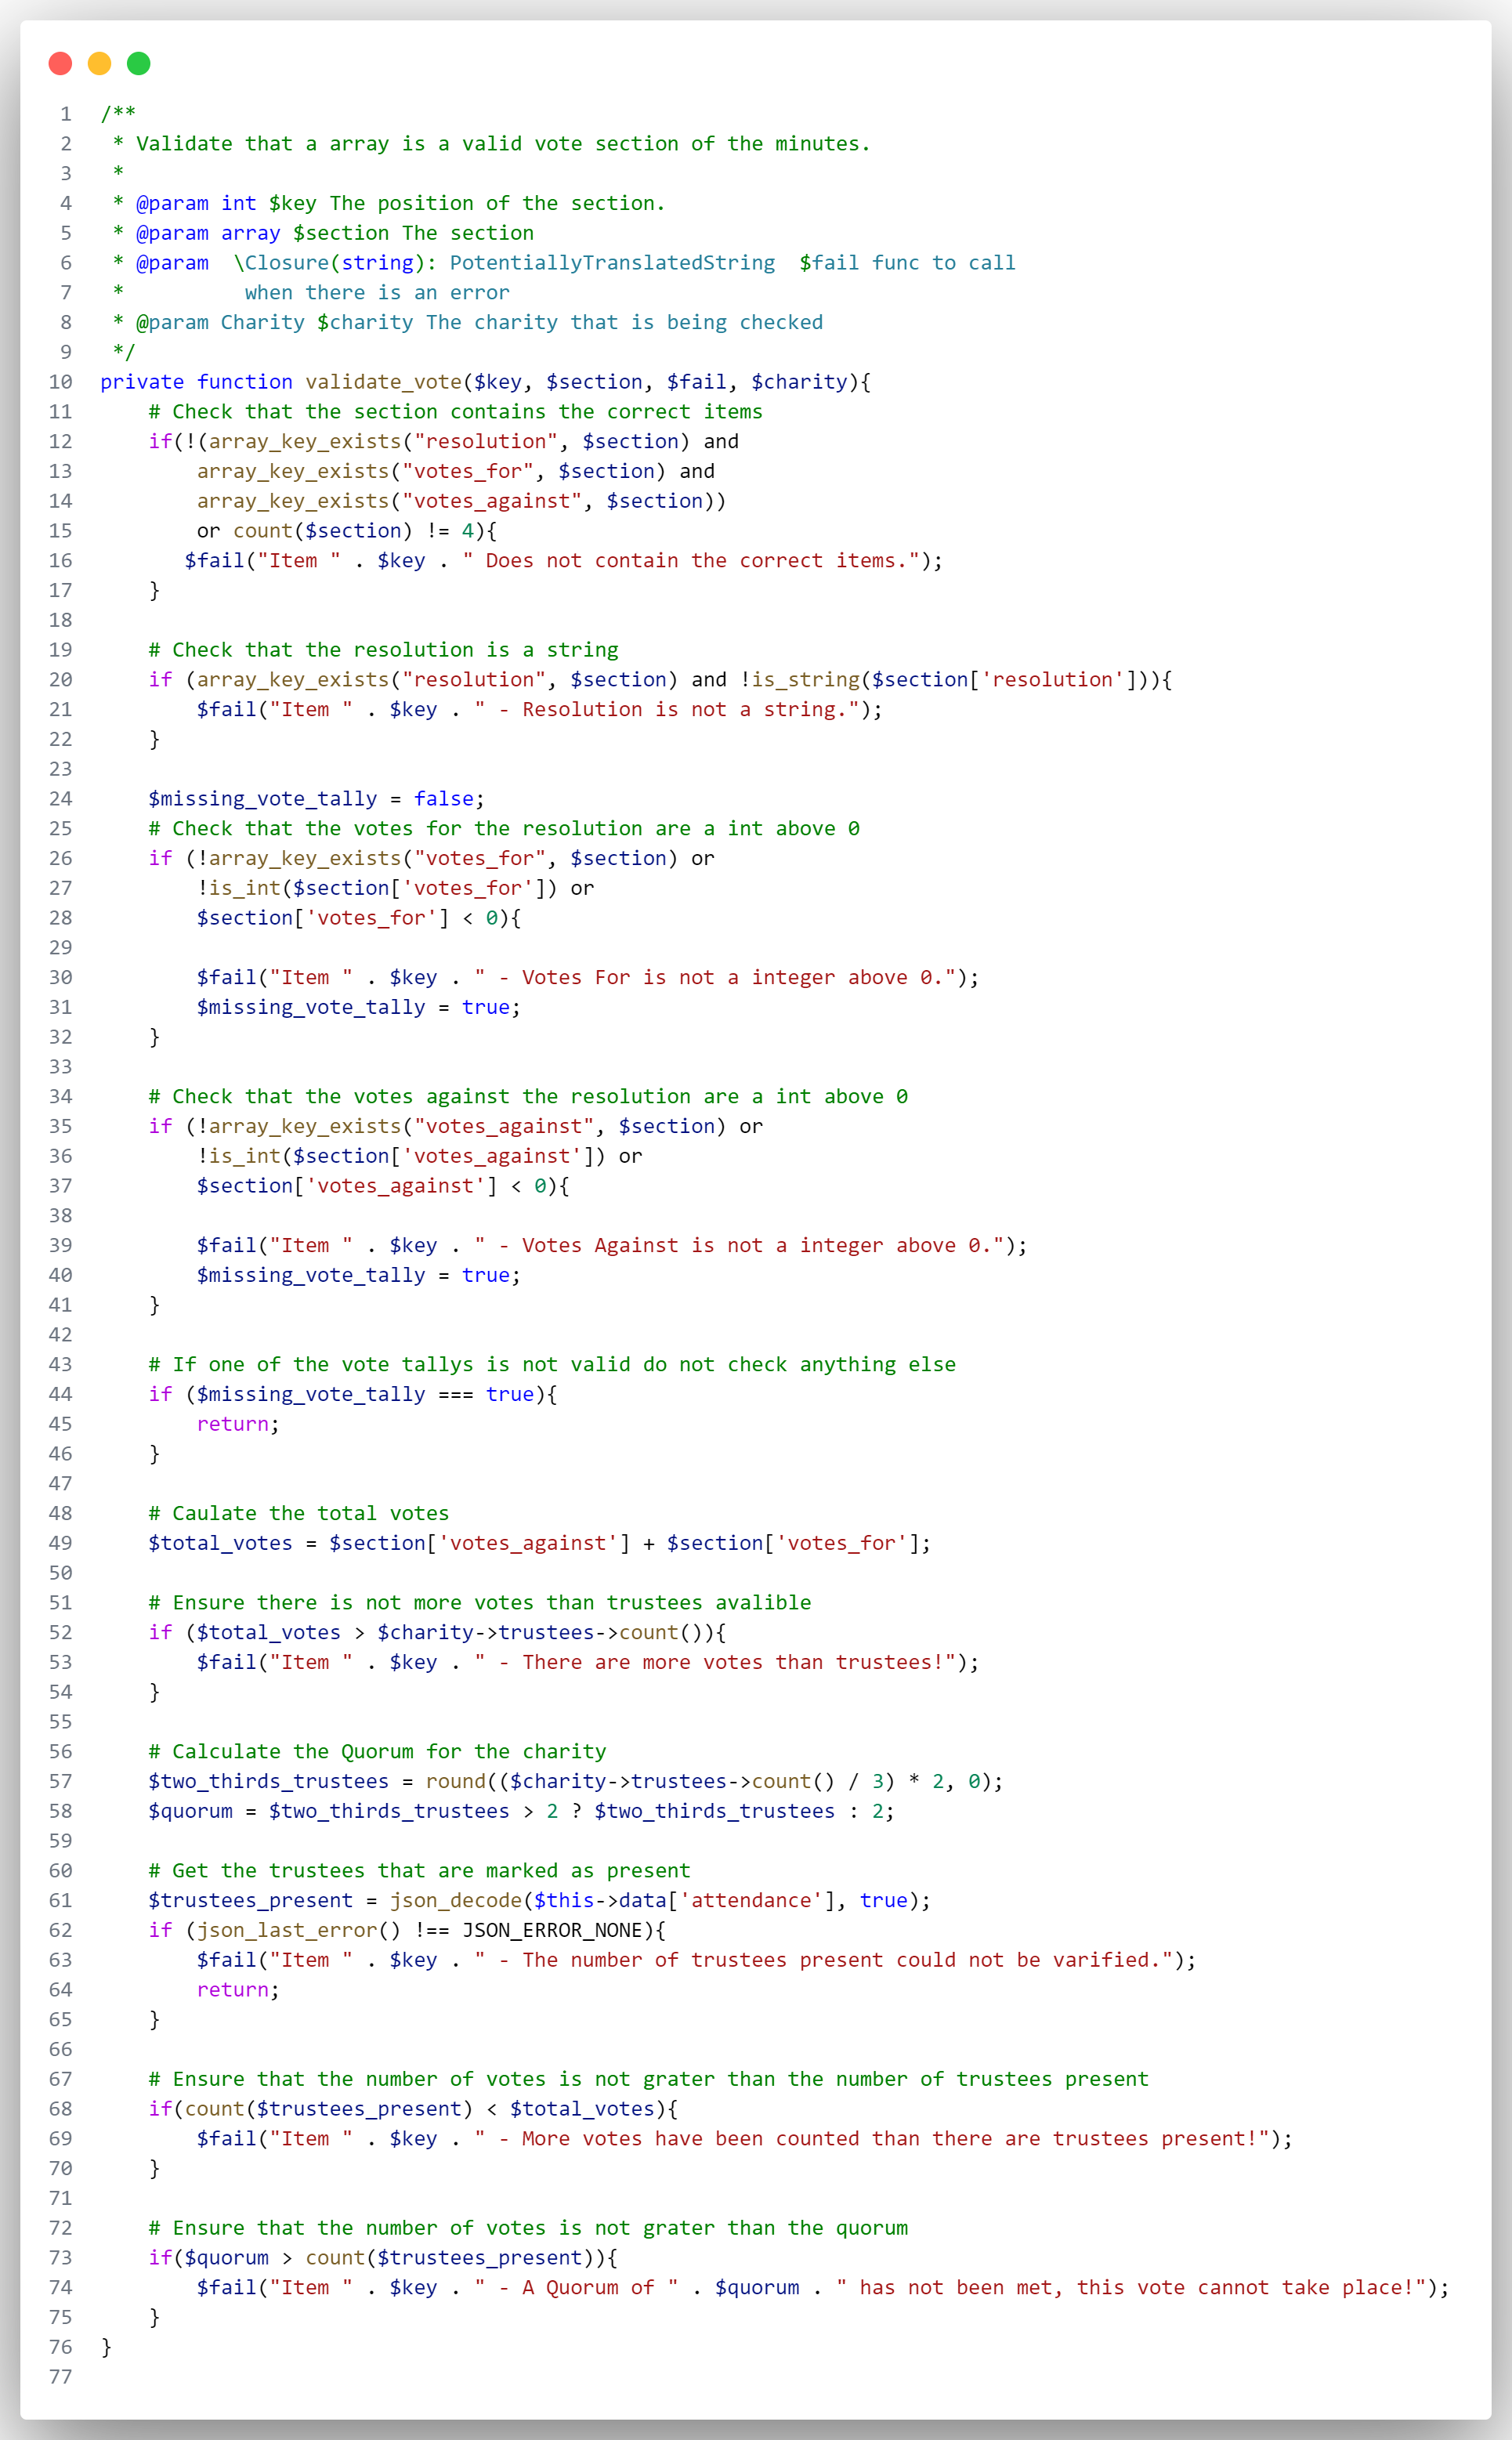
\includegraphics[width=\textwidth]{"./assets/apendix/rules-code-screenshots/Minutes - Votes v2.png"}
\end{center}
\label{fig:vote_validateion_code}
\caption{Sub function of the Minutes validation rules, validating a votes section.}
\end{figure}


\begin{figure}[H]
\begin{center}
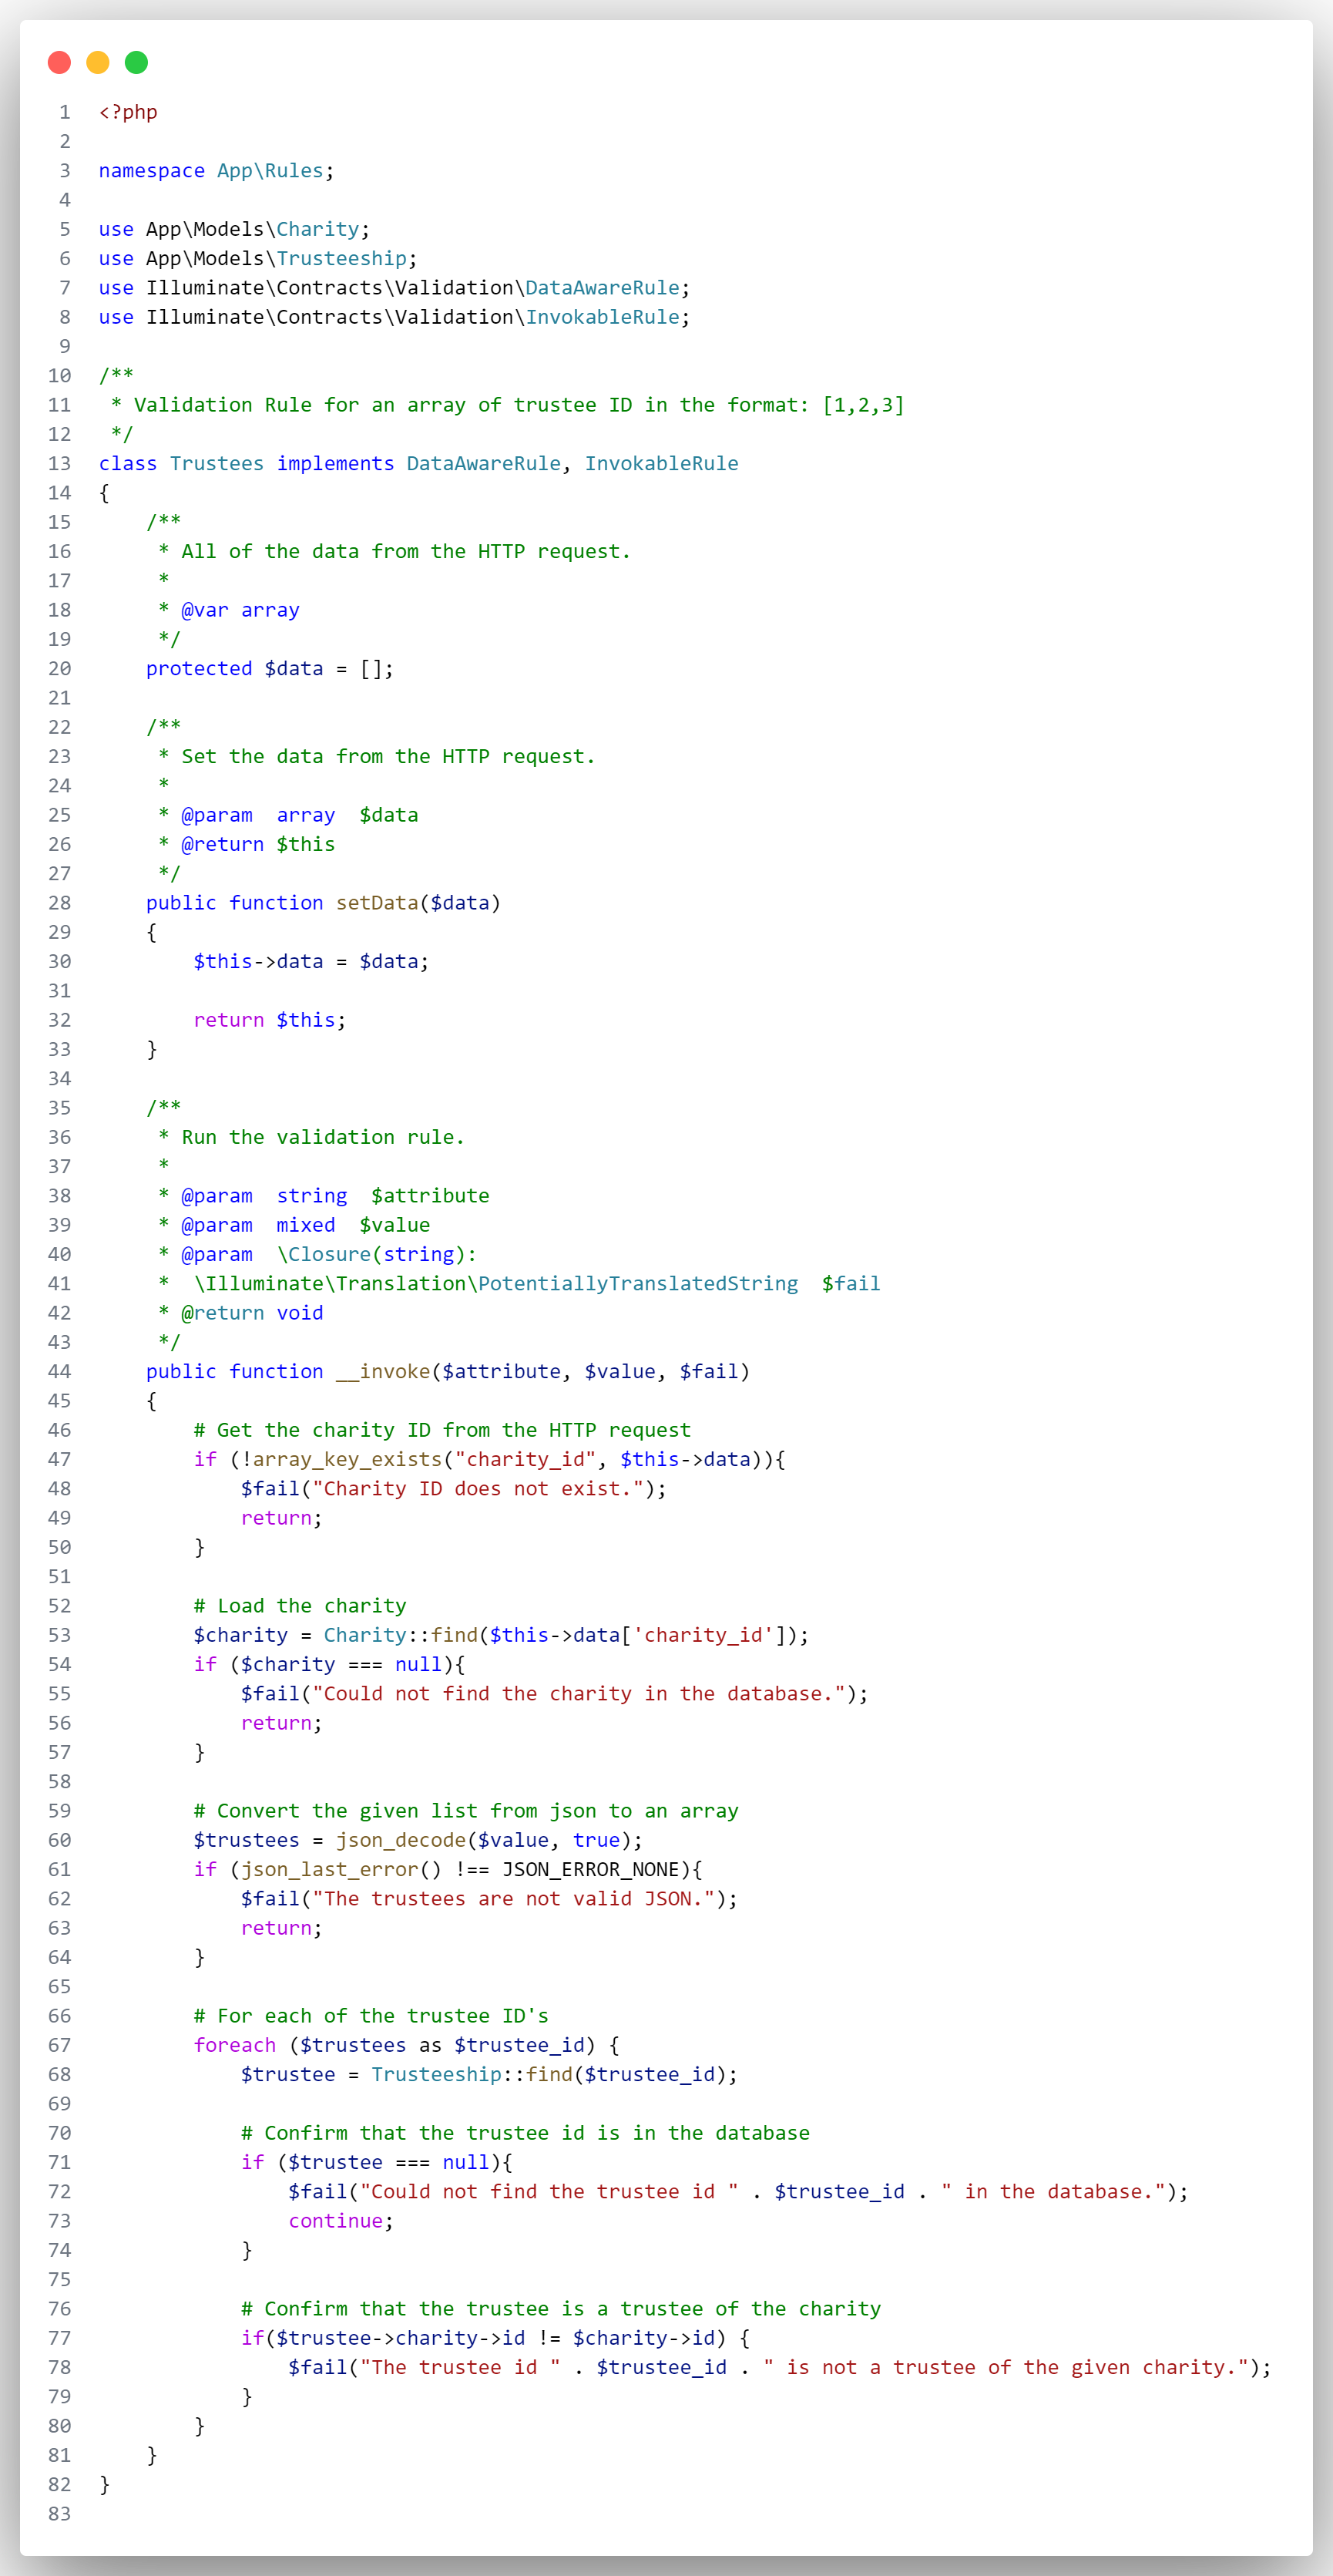
\includegraphics[width=\textwidth]{"./assets/apendix/rules-code-screenshots/Trusteeship.png"}
\end{center}
\caption{The Trustees validation rule class.}
\end{figure}

\newpage
\section{Appendix 4: Code File Structures}
\label{sec:apendix_file_strictures}

\begin{figure}[H]
\begin{center}
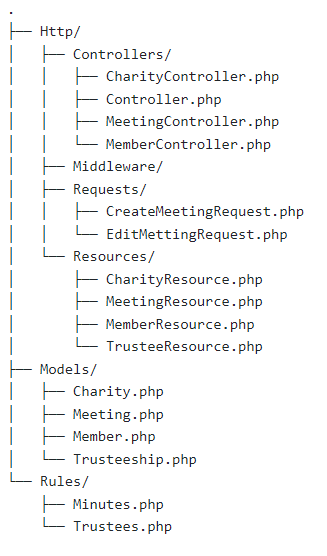
\includegraphics[]{"./assets/apendix/Laravel App File Structure.PNG"}
\end{center}
\caption{The files that have been created or modified within the base Laravel application.}
\end{figure}

\begin{figure}[H]
\begin{center}
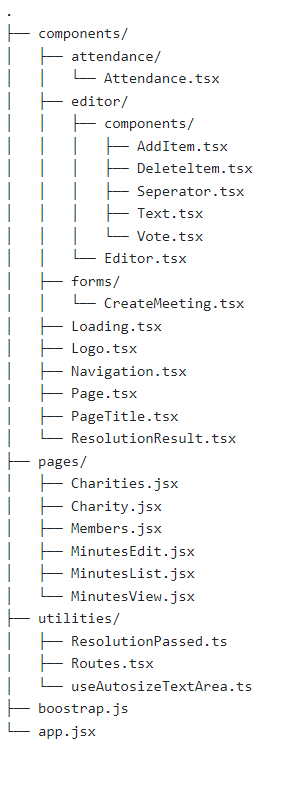
\includegraphics[]{"./assets/apendix/React App File Structure.PNG"}
\end{center}
\caption{The files that have been created within the front end React application folder.}
\end{figure}


\newpage
\section{Appendix 4: Front-end Screenshots}
\label{sec:apendix_screenshots}

\begin{figure}[H]
\begin{center}
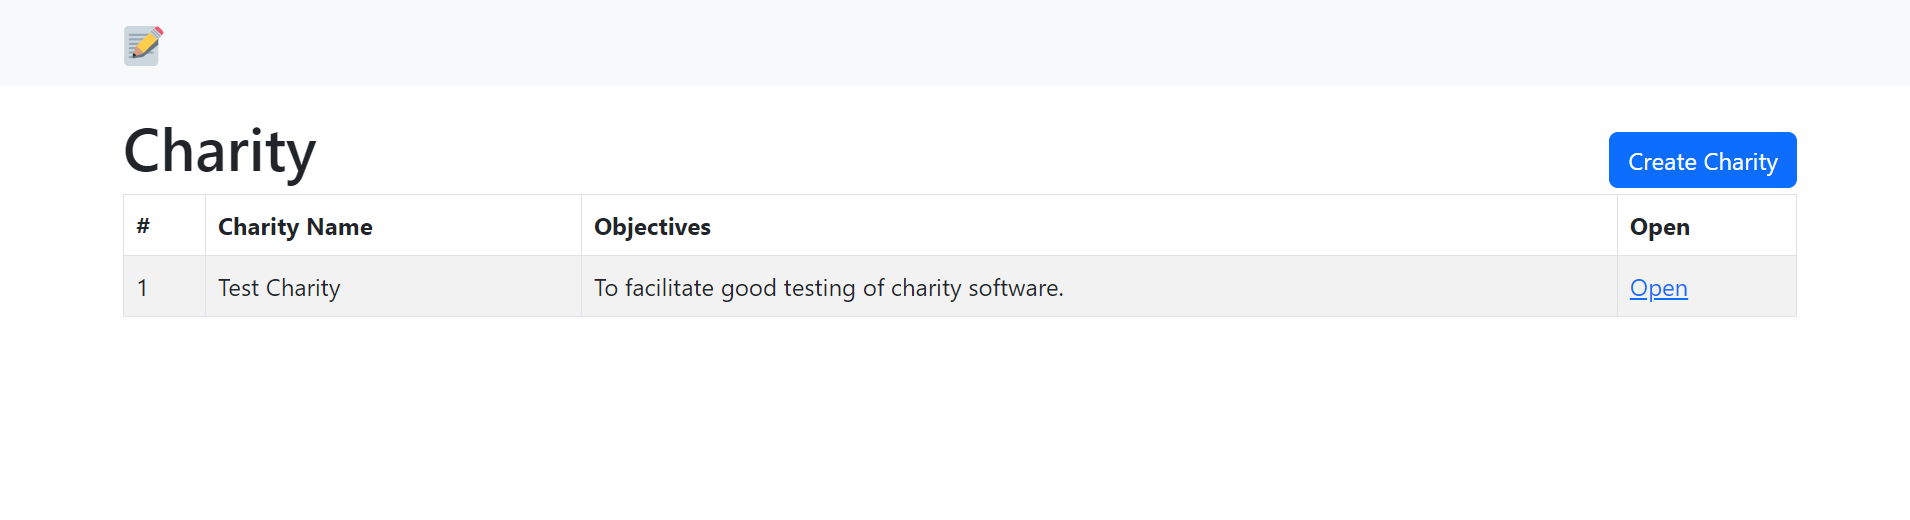
\includegraphics[width=\textwidth]{"./assets/apendix/frontend-screenshots/Charities - Cropped.png"}
\end{center}
\caption{The view of all charities.}
\end{figure}

\begin{figure}[H]
\begin{center}
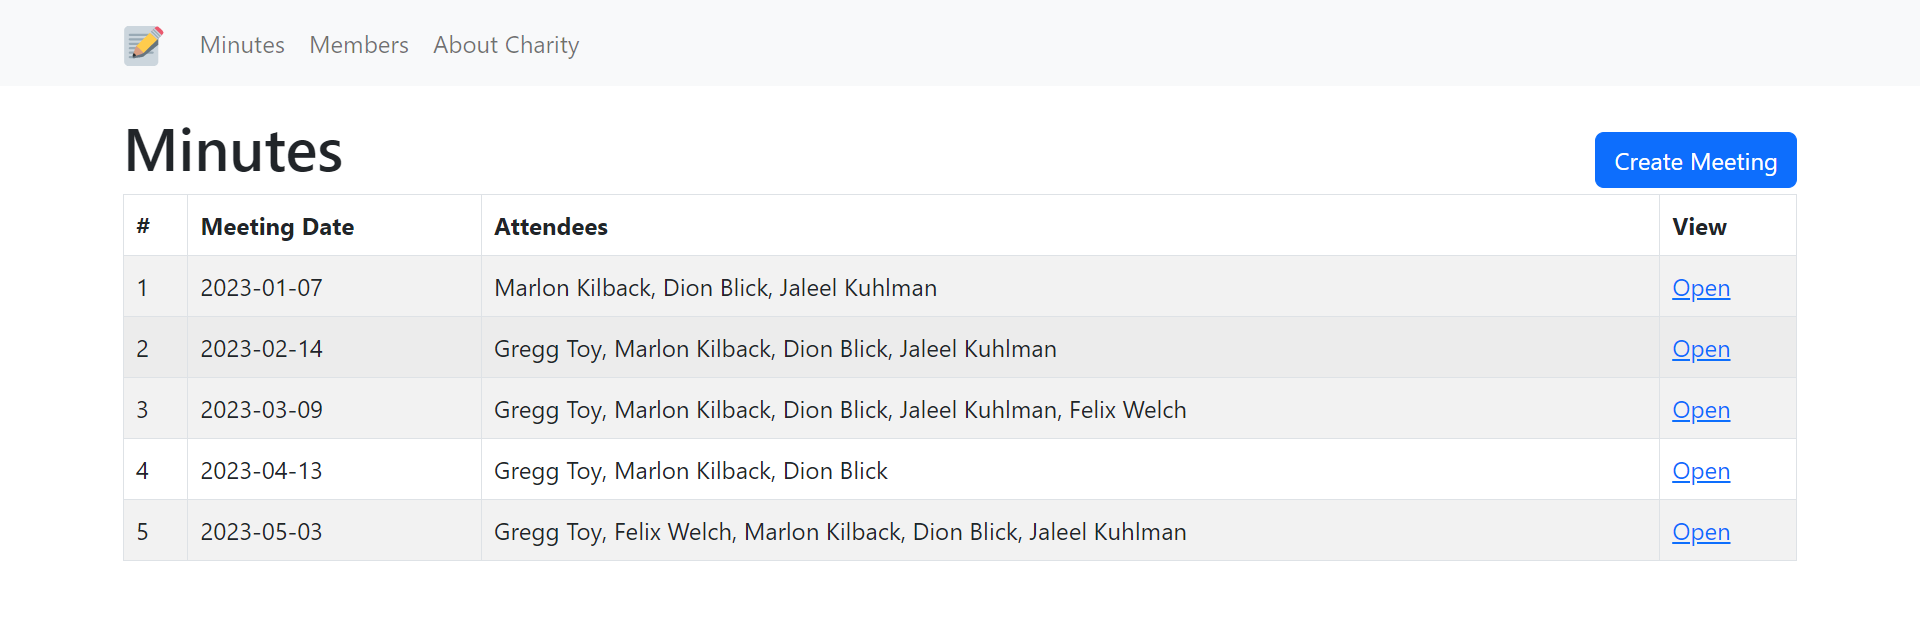
\includegraphics[width=\textwidth]{"./assets/apendix/frontend-screenshots/Minutes List - Cropped.png"}
\end{center}
\caption{The view of all minutes within a given charity.}
\end{figure}

\begin{figure}[H]
\begin{center}
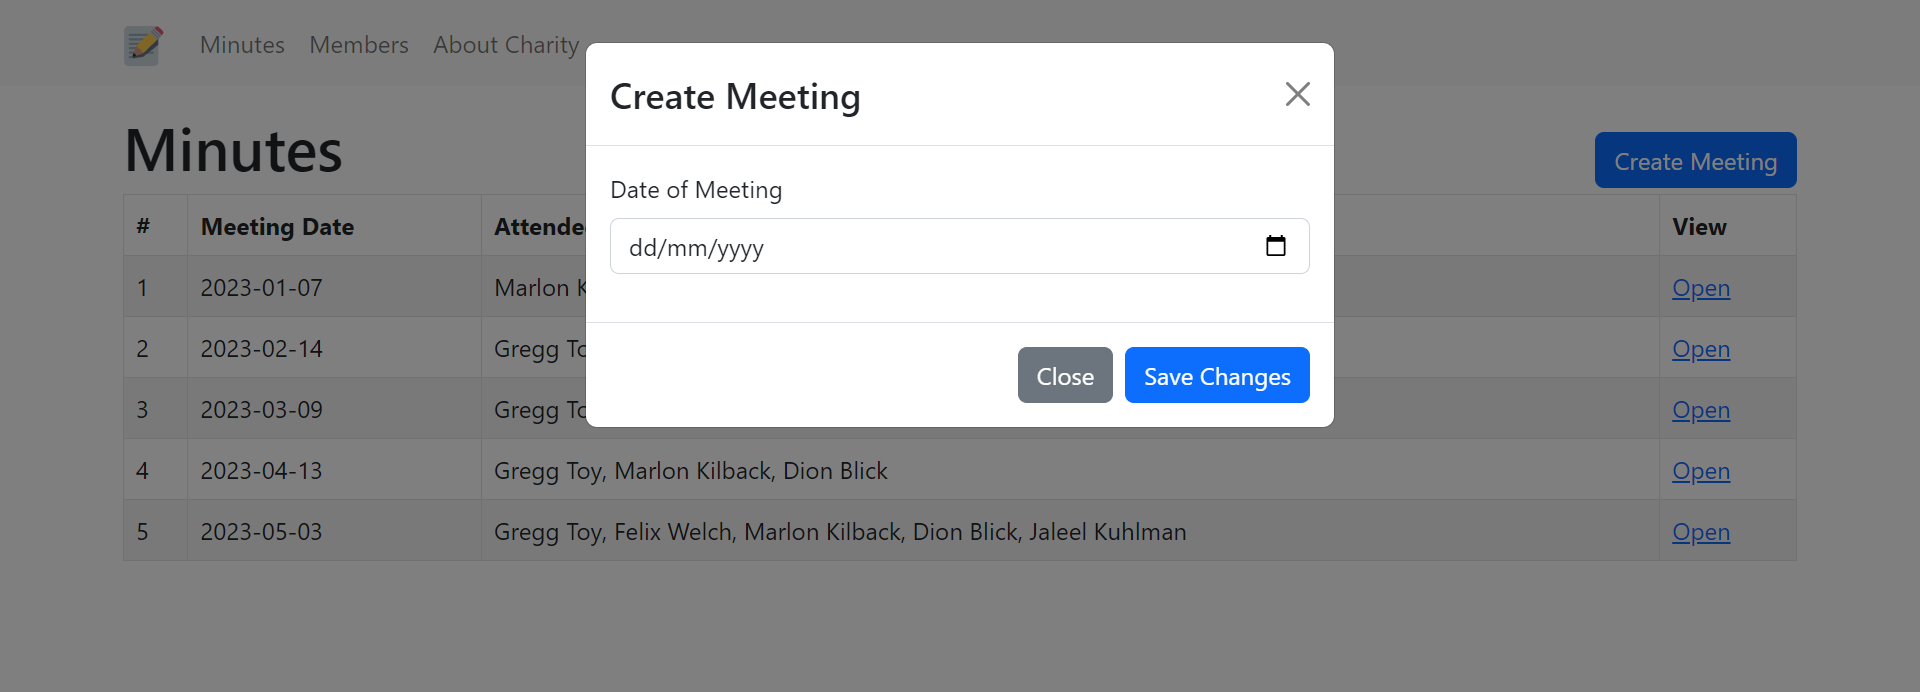
\includegraphics[width=\textwidth]{"./assets/apendix/frontend-screenshots/Minutes New - Cropped.png"}
\end{center}
\caption{The popup form to create new minutes.}
\end{figure}

\begin{figure}[H]
\begin{center}
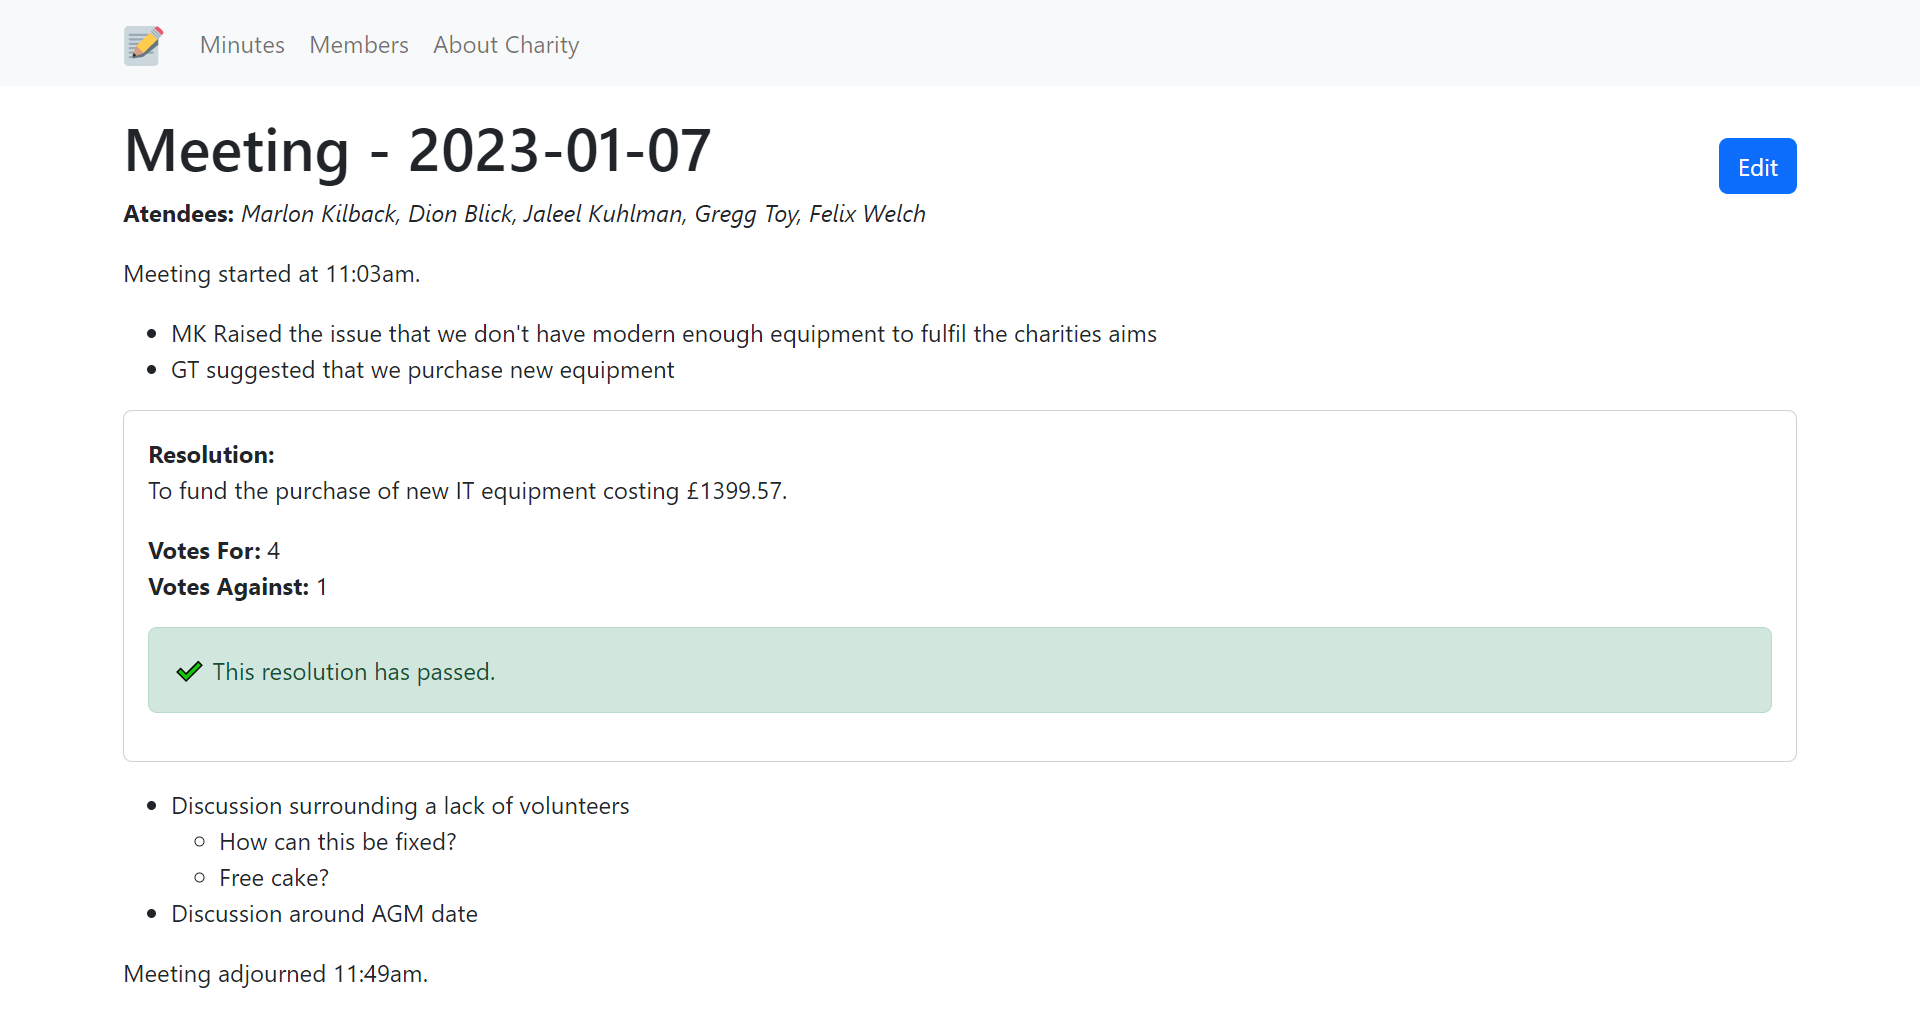
\includegraphics[width=\textwidth]{"./assets/apendix/frontend-screenshots/Minutes View.png"}
\end{center}
\caption{The page displaying the minutes of a previous meeting.}
\end{figure}

\begin{figure}[H]
\begin{center}
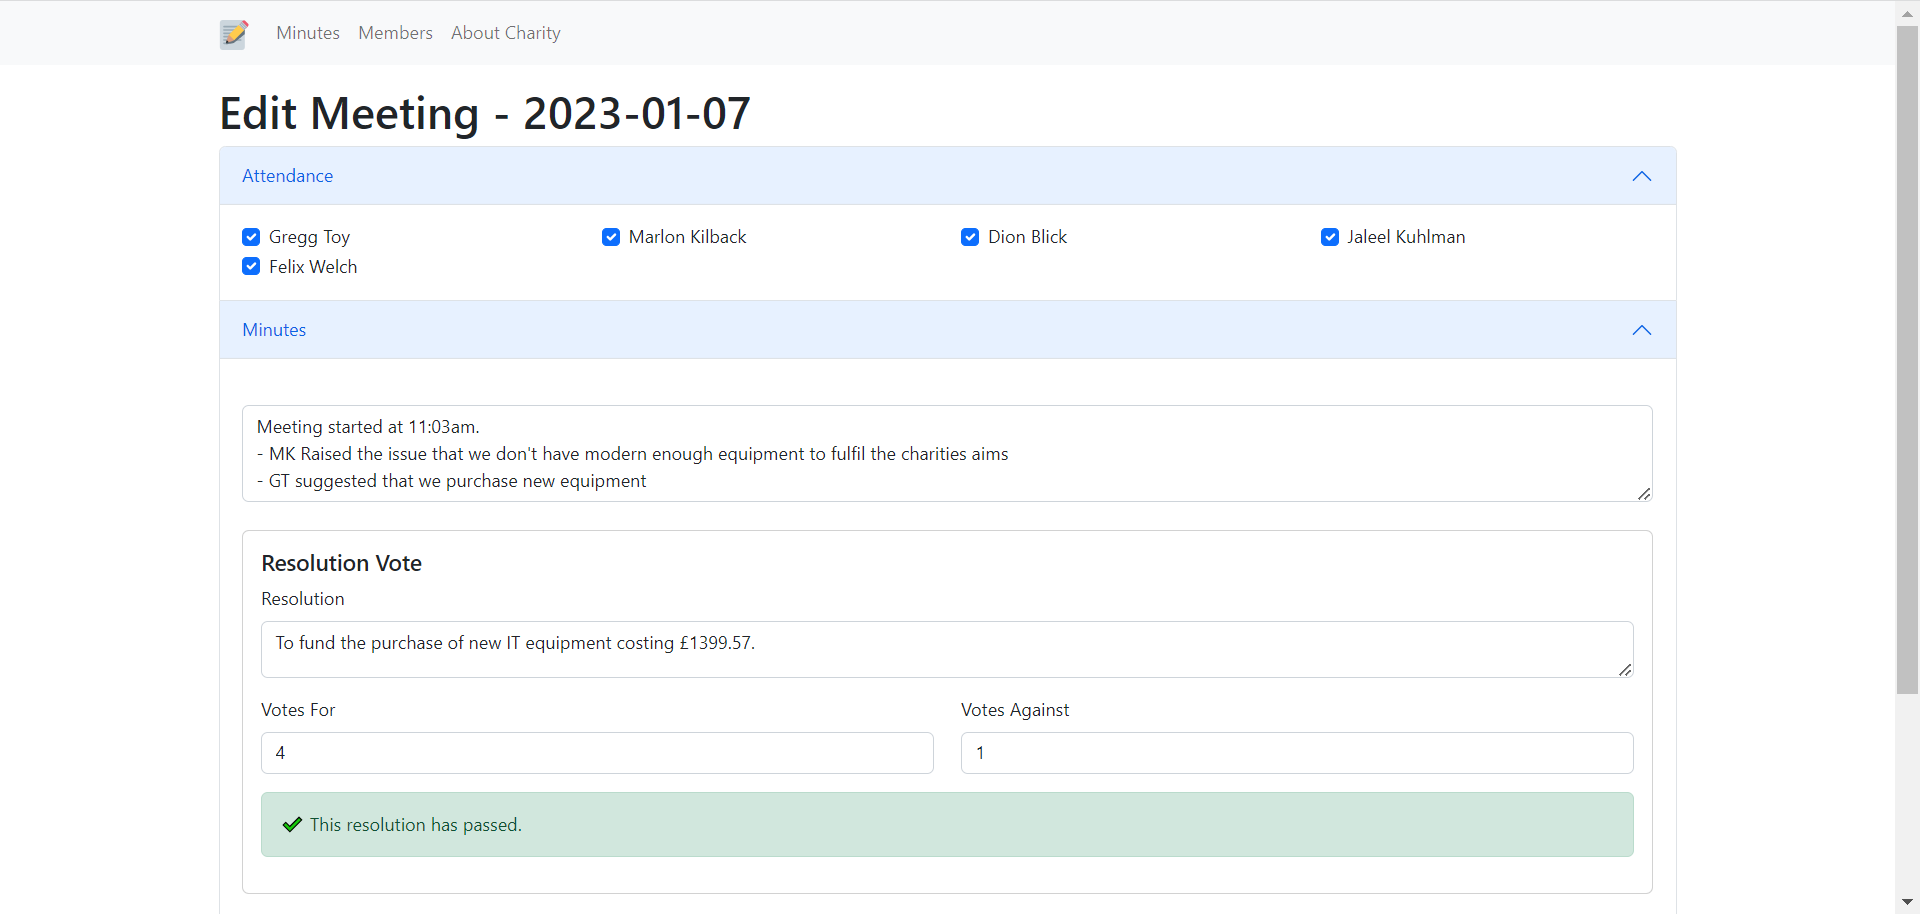
\includegraphics[width=\textwidth]{"./assets/apendix/frontend-screenshots/Minutes Edit - Overview.png"}
\end{center}
\caption{The page to edit a meeting with sections for the attendance of trustees and the minutes of the meeting.}
\end{figure}

\begin{figure}[H]
\begin{center}
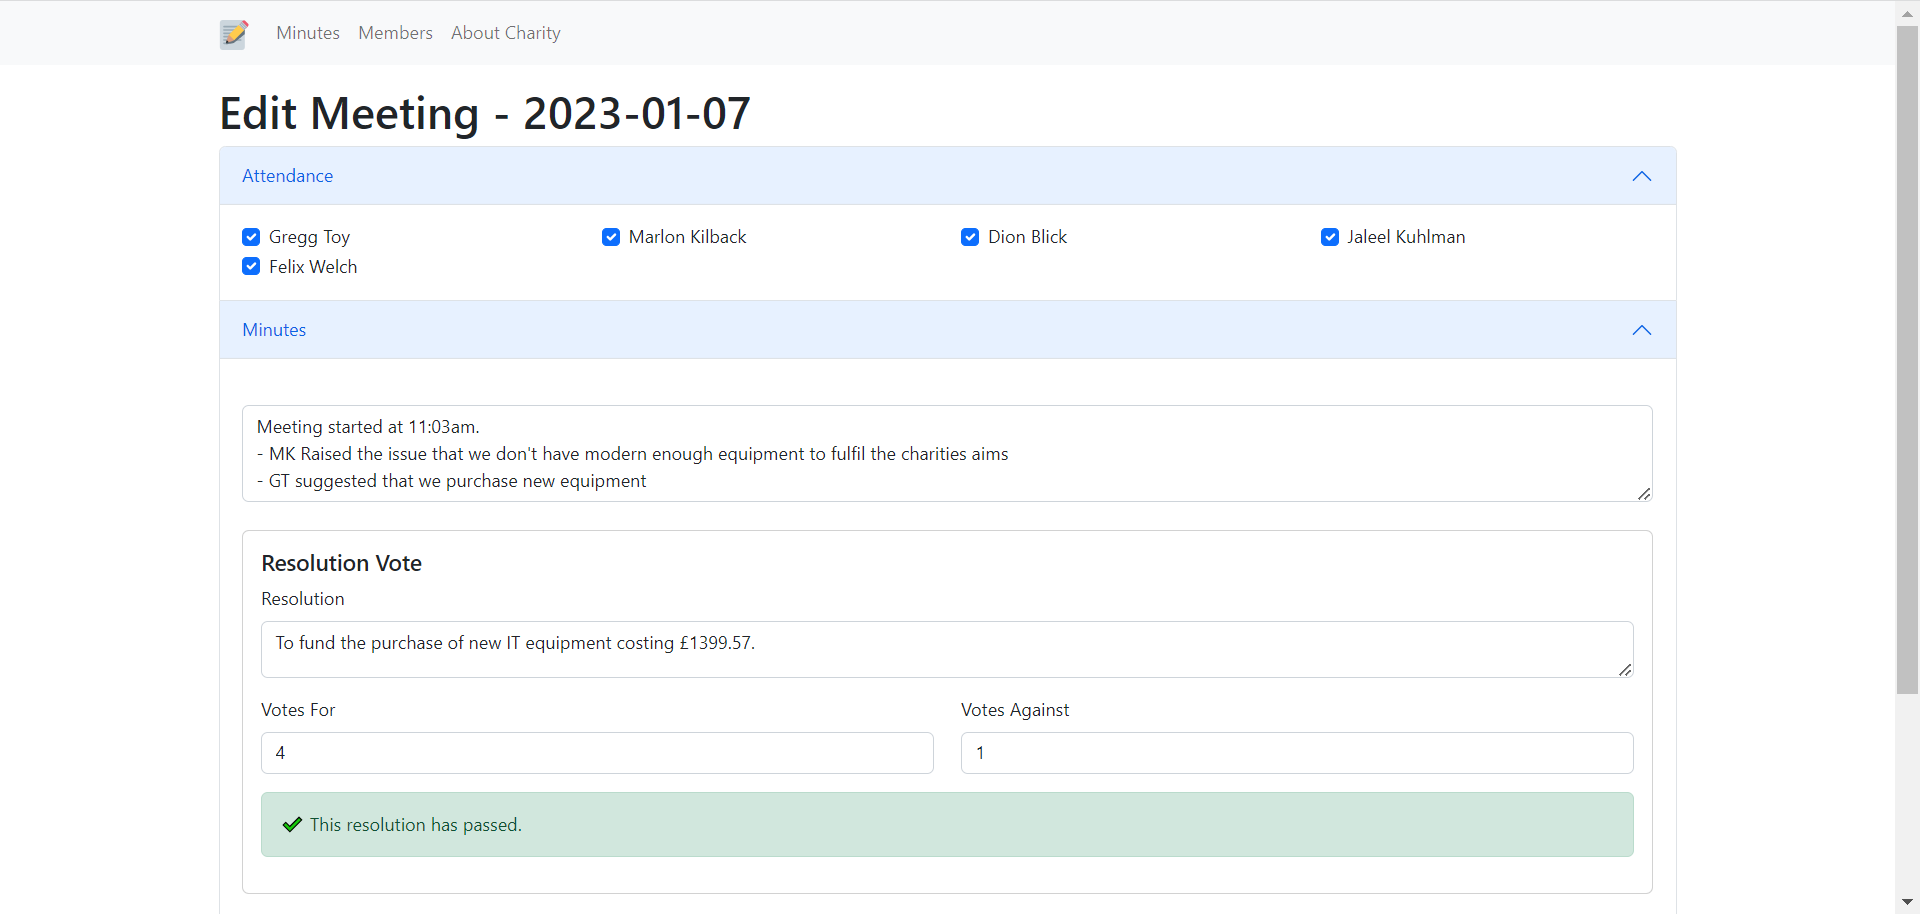
\includegraphics[width=\textwidth]{"./assets/apendix/frontend-screenshots/Minutes Edit - Overview.png"}
\end{center}
\caption{The page to edit a meeting with sections for the attendance of trustees and the minutes of the meeting.}
\end{figure}

\begin{figure}[H]
\begin{center}
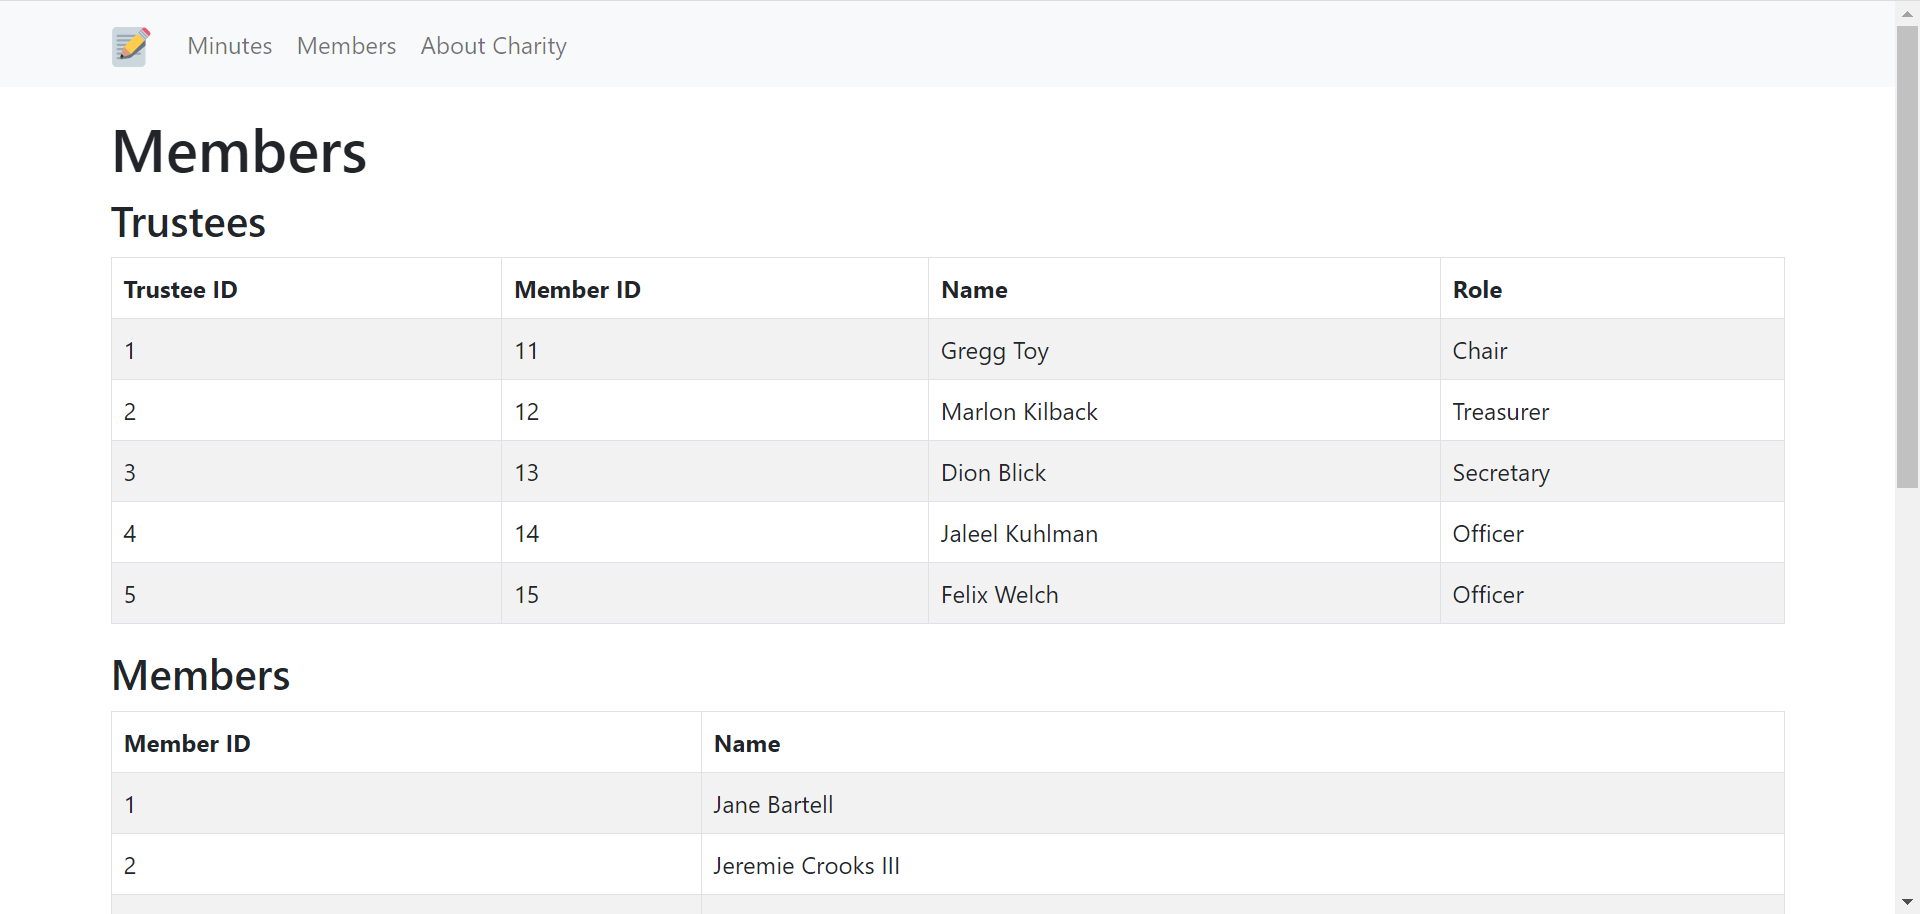
\includegraphics[width=\textwidth]{"./assets/apendix/frontend-screenshots/Members.png"}
\end{center}
\caption{A page displaying the members of a charity.}
\end{figure}

\begin{figure}[H]
\begin{center}
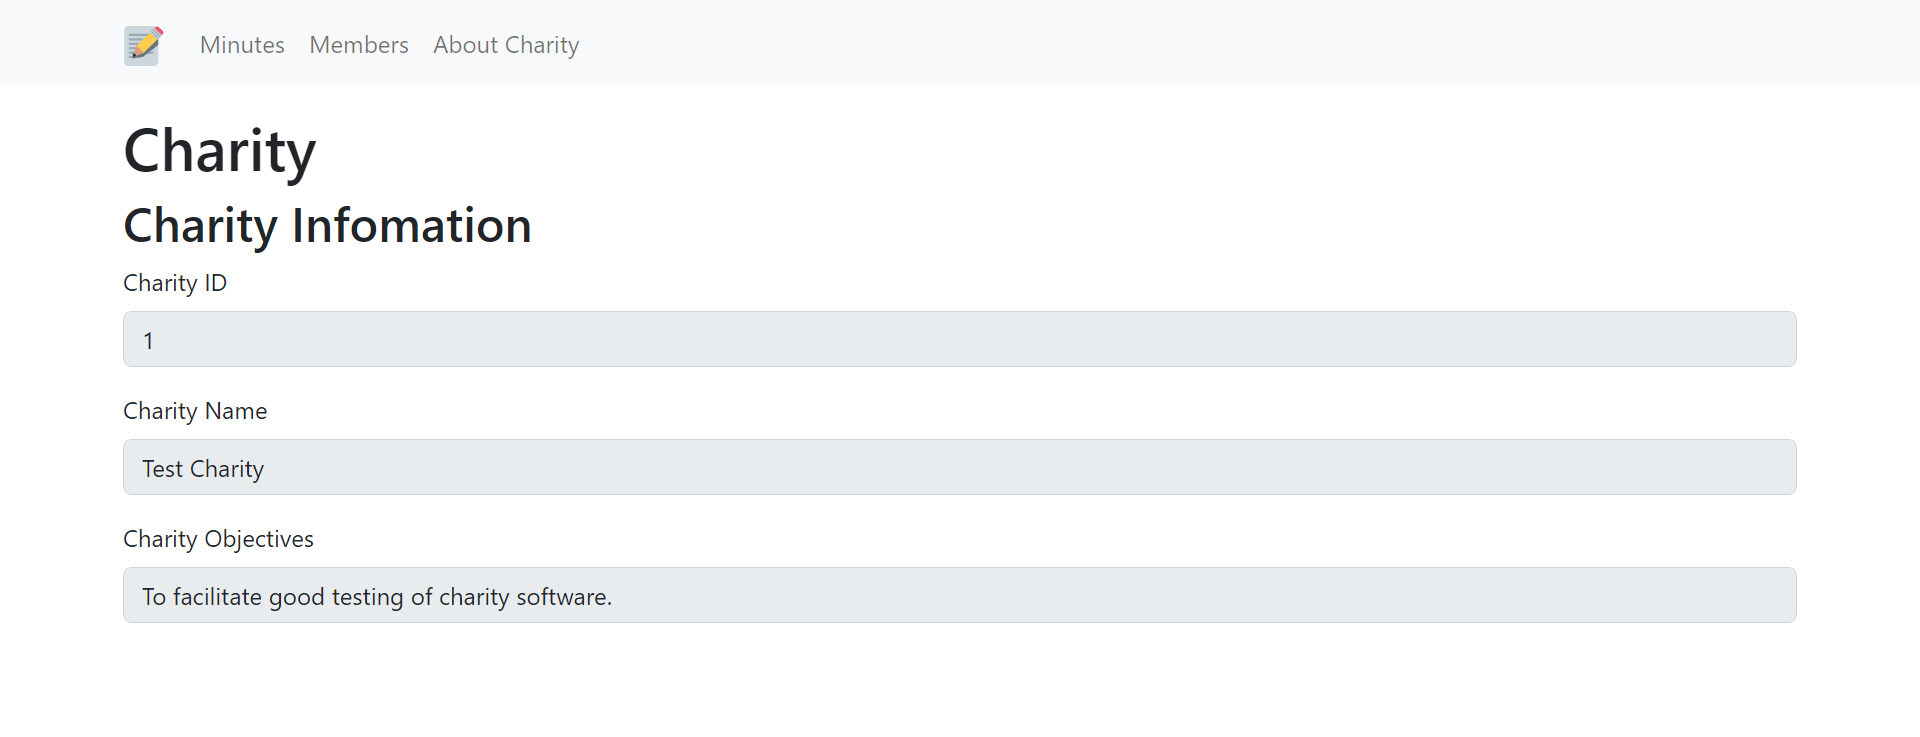
\includegraphics[width=\textwidth]{"./assets/apendix/frontend-screenshots/About Charity - Cropped.png"}
\end{center}
\caption{A page displaying an overview of the charity model.}
\end{figure}



\newpage
\section{Appendix 5: Unit Test Code Coverage Results}
\label{sec:apendix_unit_tests}

\begin{figure}[H]
\begin{center}
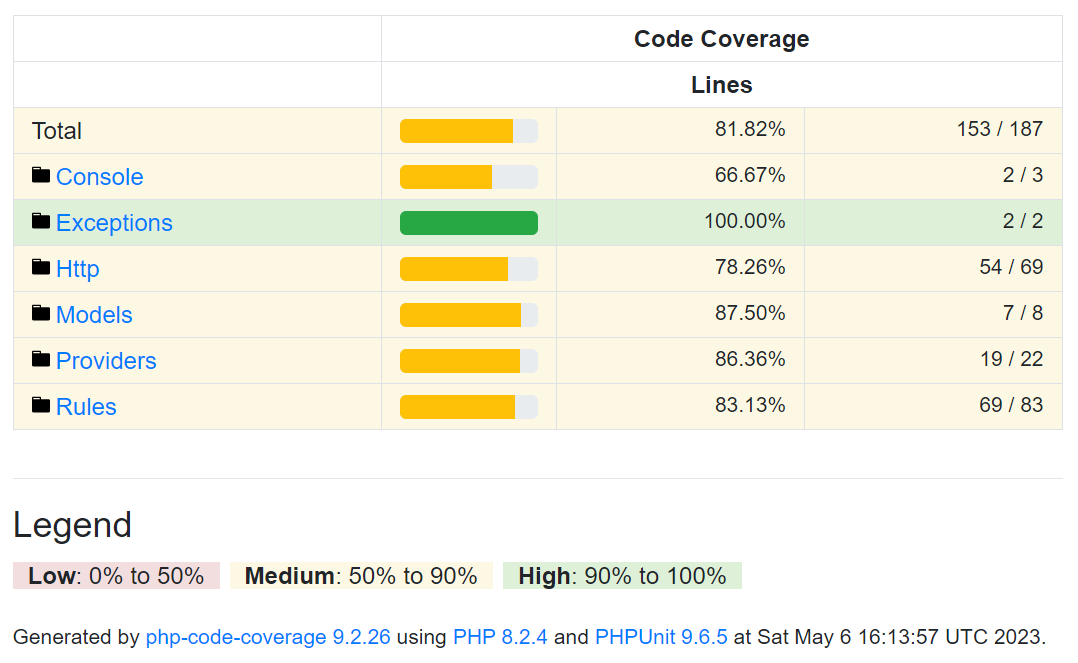
\includegraphics[width=1\textwidth]{"./assets/apendix/Code Coverage Results.PNG"}
\end{center}
\caption{Unit test code coverage results.}
\end{figure}



\printbibliography
\end{document}